\subsection{自由模中一个元素的内容}

设 A 为主理想整环，L 为自由 A-模，x 为 L 的一个元素。当 f 遍历 L 上线性形式的集合 \(L^{*}\) 时，诸元素 \(f(x)\) 构成 A 的一个理想 \(\mathfrak{c}_{\mathrm{L}}(x)\)，称为 x 在 L 中的内容。A 的元素 c 称为 x 在 L 中的一个内容，如果它生成理想 \(\mathfrak{c}_{\mathrm{L}}(x)\)；这相当于说，存在 L 上的一个线性形式 f，使得 \(f(x)=c\)，并且 c 整除 L 上每个线性形式 g 所对应的 \(g(x)\)。设 \((e_{i})_{i\in I}\) 为 L 的一组基；令 \(x=\sum a_{i}e_{i}, a_{i}\in A\)；则理想 \(\mathfrak{c}_{\mathrm{L}}(x)\) 由诸和式 \(\sum a_{i}b_{i}\) 组成，其中 \((b_{i})\) 遍历集合 \(A^{I}\)；由此立即得出，A 的元素 c 是 x 在 L 中的一个内容，当且仅当它是 x 的坐标族 \((a_{i})\) 的最大公因子。

我们称 x 是不可除元，如果 \(\mathfrak{c}_{L}(x)=\mathbf{A}\)，即 x 关于 L 的一组基的坐标整体互素。

引理1. --- 设L是主理想整环A上的自由模，且x是L的一个元素。则以下条件等价：

\begin{enumerate}
\def\labelenumi{(\roman{enumi})}
\item
  \(x\) 是不可除的；
\item
  存在一个线性形式 \(f\)，它定义在 \(L\) 上，使得 \(f(x) = 1\)；
\item
  \(x\) 非零，且子模 \(\mathbf{A}x\) 是 \(\mathbf{L}\) 的一个直因子;
\item
  \(x\) 是 \(\mathbf{L}\) 的某组基中的一个元素.
\item
  \(\Rightarrow\) (ii)：这由定义得出。
\item
  \(\Rightarrow\) (iii)：设 \(f\) 为 \(\mathbf{L}\) 上的一个线性形式，使得 \(f(x) = 1\)；则 \(x \neq 0\)，且映射 \(y \mapsto f(y)x\) 是 \(\mathbf{L}\) 的一个投影算子，其像为 \(\mathbf{A}x\).
\item
  \(\Rightarrow\) (iv)：设 \(L'\) 是 \(Ax\) 在 \(L\) 中的一个补，并设 \(B'\) 是 \(L'\) 的一组基（VII，第15页，推论2）；则 \(B' \cup \{x\}\) 是 \(L\) 的一组基.
\item
  \(\Rightarrow\) (i)：平凡。
\end{enumerate}

注记。--- 1) 若 \(x\) 是 \(L\) 中的非零元素，且 \(c\) 是 \(x\) 的一个内容，则存在唯一的元素 \(y\)（属于 \(L\)）使得 \(x = cy\)；把这个元素记作 \(x / c\)；则 \(x / c\) 是 \(L\) 的一个不可除元素。

\begin{enumerate}
\def\labelenumi{\arabic{enumi})}
\setcounter{enumi}{1}
\tightlist
\item
  内容 \(\mathfrak{c}_{\mathrm{L}}(x)\) 是挠模 \(\mathrm{L} / \mathrm{A}x\) 的零化子.
\end{enumerate}

设 L 是主理想整环 A 上的自由模，且 M 是 L 的一个子模；由 VII 第 4 页引理 1，族 \(\mathfrak{c}_{\mathrm{L}}(x)\)（\(x \in M\)）具有极大元；若 \(M \neq \{0\}\)，则这样的极大元是非零的。

命题3. --- 设L是主理想整环A上的自由模，且M是L的一个非零子模。设x是M中使 \(\mathfrak{c}_{\mathrm{L}}(x)\) 在M的各元素的内容之中为极大的一个元素，设c是x在L中的一个内容，并设f是L上的一个线性形式，使得 \(f(x) = c\).

\begin{enumerate}
\def\labelenumi{\alph{enumi})}
\item
  L 是 A(x/c) 与 f 的核 K 的直和。
\item
  \(\mathbf{M}\) 是 \(\mathbf{A}\mathbf{x}\) 与 \(\mathbf{K} \cap \mathbf{M}\) 的直和.
\item
  \(g(M) \subset Ac\) 对每个线性形式 \(g\)（\(L\) 上的）都成立。
\end{enumerate}

令 \(y = x / c\)；显然 \(\mathbf{A}y \cap \mathbf{K} = \{0\}\)，因为 \(f(y) = 1\)。此外，对每个 \(u \in L\)，我们有

\[
u = f (u) y + (u - f (u) y),
\]

其中 \(f(u) y \in \mathbf{A}y\)，且 \(u - f(u)y \in \mathbf{K}\)；这就证明了 \(a\)）。现在注意，对 \(u \in \mathbf{M}\) 我们有 \(f(u) \in \mathbf{A}c\)：事实上，设 \(u \in \mathbf{M}\)，并设 \(d\) 是 \(f(u)\) 与 \(c\) 的一个最大公因子；则存在 \(\lambda, \mu \in \mathbf{A}\) 使得 \(d = \lambda f(u) + \mu c = f(\lambda u + \mu x)\)；因而元素 \(\lambda u + \mu x\)（\(\mathbf{M}\) 中的）的内容整除 \(d\)；由 \(c\) 的极大性，这蕴含 \(d\) 与 \(c\) 相伴，从而 \(f(u) \in \mathbf{A}c\)。于是对每个 \(u\)（在 \(\mathbf{M}\) 中），我们可以写出

\[
u = (f (u) / c) x + (u - (f (u) / c) x) \in \mathrm{A} x + (\mathrm{K} \cap \mathrm{M}),
\]

这表明 \(b\)）。最后，设 \(g\) 是 \(L\) 上的一个线性形式；由 \(a\)）存在一个标量 \(\alpha \in A\) 和一个线性形式 \(h\)（\(K\) 上的），使得 \(g(u) = \alpha f(u) + h(u - f(u)y)\)；于是由 b) 我们有 \(g(\mathbf{M}) \subset \mathbf{A}c + h(\mathbf{K} \cap \mathbf{M})\)。因此要证明 c)，只需证明对 K 上的每个线性形式 h 都有 \(h(\mathbf{K} \cap \mathbf{M}) \subset \mathbf{A}c\)，或等价地，对 L 上满足 \(h(x) = 0\) 的每个线性形式 h 成立；现在，若 \(u \in K \cap M\) 且 d 是 \(h(u)\) 与 c 的一个最大公因子，则存在 \(\lambda\)、\(\mu \in A\) 使得 \(d = \lambda h(u) + \mu c\)；则 \((f + h)(\lambda u + \mu x) = d\)，这如上所述蕴含 \(h(u) \in Ac\)，从而 c) 成立。

\subsection{子模的不变因子}

定理1. --- 设L是主理想整环A上的自由模，且设M是L的秩 n 为有限的子模。则存在L的一组基B、B 中的 n 个元素 \(e_{i}\)，以及 A 的 n 个非零元素 \(\alpha_{i}\)（\(1 \leqslant i \leqslant n\)），使得：

\begin{enumerate}
\def\labelenumi{\alph{enumi})}
\item
  诸 \(\alpha_{i}e_{i}\) 构成 \(\mathbf{M}\) 的一组基;
\item
  \(\alpha_{i}\) 整除 \(\alpha_{i + 1}\)，其中 \(1\leqslant i\leqslant n - 1\)
\end{enumerate}

此外，由 \((e_{i})\) 生成的模 M' 以及诸主理想 \(A\alpha_{i}\) 都由上述条件唯一确定；模 M'/M 是 L/M 的挠子模，并且同构于诸 A-模 A/A \(\alpha_{i}\) 的直和；最后，L/M 是 M'/M 与一个同构于 L/M' 的自由模的直和。

\begin{enumerate}
\def\labelenumi{\arabic{enumi})}
\tightlist
\item
  \(e_i\) 与 \(\alpha_i\) 的存在性.
\end{enumerate}

如果 \(M = \{0\}\)，那么定理是平凡的。如果 \(M \neq \{0\}\)，则由命题3可知，存在 L 的一个元素 \(e_{1}\)、A 的一个非零元素 \(\alpha_{1}\) 以及 L 的一个子模 \(L_{1}\)，使得 L 是 \(Ae_{1}\) 与 \(L_{1}\) 的直和，使得 M 是 \(A\alpha_{1}e_{1}\) 与 L 的子模 \(M_{1} = M \cap L_{1}\) 的直和，并且使得对 L 上的每个线性形式 g 都有 \(g(M) \subset A\alpha_{1}\)。

现在我们可以对 \(n\)（即 \(M\) 的秩）进行归纳。由于 \(L_1\) 是自由模（VII，第 15 页，推论 2），且 \(M_1\) 的秩为 \(n - 1\)，故存在一组基 \(B_1\)（\(L_1\) 的）、\((n - 1)\) 个元素 \(e_2, \ldots, e_n\)（取自 \(B_1\)），以及非零元素 \(\alpha_2, \ldots, \alpha_n\)（\(A\) 中的），使得 \((\alpha_2e_2, \ldots, \alpha_ne_n)\) 是 \(M_1\) 的一组基，且 \(\alpha_i\) 整除 \(\alpha_{i+1}\)，其中 \(2 \leqslant i \leqslant n - 1\)。若 \(L'\) 是 \(L_1\) 的由 \(B_1\) 中异于 \(e_2, \ldots, e_n\) 的元素生成的子模，则 \(L\) 是 \(L'\) 与模 \(M'\)（由 \(e_1, \ldots, e_n\) 生成的）的直和；而 \((e_1, \ldots, e_n)\) 是 \(M'\) 的一组基，且 \((\alpha_1e_1, \ldots, \alpha_ne_n)\) 是 \(M\) 的一组基。现在只需证明 \(\alpha_1\) 整除 \(\alpha_2\)；但 \(A\alpha_2\) 具有形式 \(g(M_1)\)，其中 \(g\) 是 \(L\) 上由 \(g(e_2) = 1\)、\(g(e_i) = 0\)（\(i \neq 2\)）以及 \(g(L') = \{0\}\) 定义的线性形式；而我们上面已经看到 \(g(M_1) \subset A\alpha_1\).

2) 唯一性性质。

由于诸 \(\alpha_{i}\) 非零，模 \(\mathbf{M}'\) 是由那些 \(x\in L\)（使得 \(\beta x\in M\) 对 A 中某个 \(\beta \neq 0\) 成立）组成的集合；换言之，\(\mathbf{M}' / \mathbf{M}\) 是 L/M 的挠子模。这就唯一确定了 \(\mathbf{M}'\)。

显然 \(M^{\prime}/M\) 同构于 n 个循环模 \(A/A\alpha_{i}\) 的直和（II，第 204 页，公式 (26)）。设 r 为异于 A 的理想 \(A\alpha_{i}\) 的个数：于是前 n−r 个理想 \(A\alpha_{i}\) 等于 A，而后 r 个异于 A。则 \(M^{\prime}/M\) 也同构于诸模 \(A/A\alpha_{n}, \ldots, A/A\alpha_{n-r+1}\) 的直和，其中 \(A\alpha_{n} \subset A\alpha_{n-1} \subset \ldots \subset A\alpha_{n-r+1} \neq A\).

于是 VII 第 16 页命题 2 的推论的条件得到满足：诸理想 \(\mathbf{A}\alpha_{i}\)（\(1 \leqslant i \leqslant n\)）从而由模 \(\mathbf{M}'/\mathbf{M}\) 唯一确定.

由于 L 是 \(M'\) 与 \(L'\) 的直和，故 L/M 是 \(M'/M\) 与 \((L'+M)/M\) 的和，且这个和是直和，因为 \((L'+M) \cap M' = M\)；另一方面，\((L'+M)/M\) 同构于 \(L'/(M \cap L')\)（I，第 41 页，定理 4，c)），即同构于 \(L'\)，这表明 \((L'+M)/M\) 是一个自由模，同构于 \(L/M'\).

推论。--- 主理想整环 A 上的自由模 L 中秩有限的子模 M 在 L 中有补，当且仅当 L/M 是无挠的。

在定理1的记号下，若 L/M 是无挠的，则 \(M = M'\)，且 \(M'\) 在 L 中有补 \(L'\)。反之，若 M 在 L 中有补 \(L'\)，则 L/M 同构于 \(L'\)，它是自由的（VII，第 15 页，推论 2），从而更是无挠的。

注记. --- 可能发生这样的情形：自由模 L 中的无限秩子模 M 可使 L/M 是无挠的，但 M 在 L 中没有补（VII，第 60 页，习题 6，b)）。

定义1.——在定理1的记号与假设下，A 的诸理想 \(A\alpha_{i}\) 称为子模 M 关于模 L 的不变因子。

当 A 是有理整数环 Z 或域 K 上一个未定元的多项式环 K{[}X{]} 时，有一种为 A 的每个理想典范地选取生成元的方式：在 Z 的情形取正整数，在 K{[}X{]} 的情形取首一多项式（VII，第 5 页）。在每一种情形下，不变因子 \(A\alpha_{i}\) 的典范生成元（滥用术语）也称为 M 关于 L 的一个不变因子。

\subsection{有限生成模的结构}

定理2.——设A为主理想整环，则每个有限生成的A-模E都同构于有限多个（m 个）循环模 \(A/a_{k}\) 的直和，其中 \(a_{k}\) 是 A 的理想（其中某些可以为零），满足 \(a_{1} \subset a_{2} \subset \ldots \subset a_{m} \neq A\)，并且这些理想由上述条件唯一确定。

如果 E 可由 q 个元素生成，则它同构于一个商模 L/M，其中 \(L = A^{q}\)（II，第 218 页）。由于 M 具有有限秩 \(n \leqslant q\)（VII，第 15 页，命题 1），定理 1（VII，第 18 页）的条件得到满足。于是在定理 1 的记号下，L/M 同构于 \(L'\)（\(M'\) 在 L 中的一个补）与挠模 \(M'/M\) 的直和。模 \(L'\) 是秩为 p = q − n 的自由模，故同构于 \(A^{p}\)。若 r 是使 \(A\alpha_{r} \neq A\) 的最小指标，则 \(M'/M\) 同构于诸模 \(A/A\alpha_{i}\)（\(r \leqslant i \leqslant n\)）的直和。于是，若取 \(m = p + (n - r + 1)\)、\(\mathfrak{a}_{k} = (0)\)（\(1 \leqslant k \leqslant p\)）以及 \(\mathfrak{a}_{p+j} = A\alpha_{n-j+1}\)（\(1 \leqslant j \leqslant n - r + 1\)），则所述条件即得到满足。唯一性由 VII 第 16 页的推论得出。

\pandocbounded{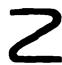
\includegraphics[keepaspectratio]{images/part003_91527dd3.jpg}}

推论 1. --- 主理想整环上的每个有限生成模 E 都是 E 的挠子模与一个自由模的直和。

E 的挠子模一般有若干个不同的补。例如，若 \(E = \mathbf{Z} \times (\mathbf{Z}/(2))\)，则 E 的挠子模为 \(\{0\} \times (\mathbf{Z}/(2))\)；它有一个补 \(Z \times \{0\}\)，也有由所有形如 \((n, \bar{n})\) 的元素组成的子模，其中 n 遍历 Z，\(\bar{n}\) 是 n 模 2 的剩余类。

推论 2. --- 主理想整环上的每个无挠有限生成模都是有限秩的自由模。

这直接由推论1得出。

\pandocbounded{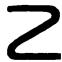
\includegraphics[keepaspectratio]{images/part003_b18cf4bc.jpg}}

模为有限生成的这一条件是本质的。例如，A 的分式域 K 的加法群作为 A-模是无挠的；然而当 \(A \neq K\) 时它不是自由模，因为一方面 K 的任意两个元素都有一个公因子，另一方面 K 不是循环 A-模，否则 \(K = ab^{-1}A\)（\(a, b \in A\)），从而 \(b^{-2} = acb^{-1}\)（\(c \in A\)），于是 \(b^{-1} = ac \in A\)，即 K = A。

定义2. --- 在定理2的记号与假设下，理想 \(\mathfrak{a}_k\) 称为模E的不变因子。

正如定义 1（VII，第 19 页）那样，当 A = Z 或 A = K{[}X{]} 时，理想 \(a_{k}\) 的典范生成元（正整数或首一多项式）（滥用术语）也称为有限生成模 E 的一个不变因子。

\pandocbounded{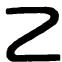
\includegraphics[keepaspectratio]{images/part003_8ba9a087.jpg}}

我们必须小心，不要将模 E 的不变因子与自由模 L 的子模 M 关于模 L 的不变因子（定义 1）混淆。

\subsection{不变因子的计算}

命题4. --- 设 A 为主理想整环，L 为具有有限基 \((u_{j})\) \((1 \leqslant j \leqslant k)\) 的自由 A-模，设 M 是 L 的一个子模，设 \((x_{i})\) 是 M 的一个生成元组，并设 \(A\alpha_{i}\) \((1 \leqslant i \leqslant n)\) 是 M 关于 L 的不变因子。则对 \(1 \leqslant m \leqslant n\)，乘积 \(\delta_{m} = \alpha_{1} \ldots \alpha_{m}\) 是以诸 \(x_{i}\) 关于基 \((u_{j})\) 的坐标向量为列的矩阵的 m 阶子式的一个最大公因子。

由定理 1 显然可知 \(M \subset \alpha_{1}L\)，因而 M 中任何元素的坐标都是 \(\alpha_{1}\) 的倍数。另一方面，存在 M 的一个元素 x，使 \(\alpha_{1}\) 是 x 在 L 中的一个内容。把 x 表示成诸 \(x_{t}\) 的线性组合，便知 \(\alpha_{1}\) 属于由诸 \(x_{t}\) 的坐标生成的理想。由于这些坐标都是 \(\alpha_{1}\) 的倍数，于是 \(\alpha_{1}\) 确是它们的最大公因子，从而我们的断言在 m = 1 的情形得证。

对于一般的 \(m\)，考虑 M 的第 \(m\) 个外幂 \(\Lambda\) M（III，第 507 页）。在定理 1 的记号下，存在 M 的一组基 \((a_i)\)，其中 \(a_i = \alpha_i e_i\)（\(1 \leqslant i \leqslant n\)）；于是 \(\Lambda\) M 有一个由诸元素 \(a_{i_1} \wedge \ldots \wedge a_{i_m}\) 组成的基，其中 \((i_1, \ldots, i_m)\) 遍历由 \(m\) 个取自 \((1, n)\) 的元素组成的严格递增序列的集合。而诸元素 \(e_{i_1} \wedge \ldots \wedge e_{i_m}\) 属于一组基 \(B_m\)（\(\bigwedge^m L\) 的基）。因此从 \(\bigwedge^m M\) 到 \(\bigwedge^m L\) 的典范映射是从 \(\bigwedge^m M\) 到 \(\bigwedge^m L\) 的某个子模上的一个同构，该子模以诸元素 \((\alpha_{i_1} \ldots \alpha_{i_m}) e_{i_1} \wedge \ldots \wedge e_{i_m}\) 为基，我们把这个子模与 \(\bigwedge^m M\) 等同起来。由于 \(\alpha_j\) 是 \(\alpha_k\) 的倍数（对 \(j \geqslant k\)），诸元素 \(\alpha_{i_1} \ldots \alpha_{i_m}\) 都是 \(\delta_m = \alpha_1 \ldots \alpha_m\) 的倍数，且其中之一等于 \(\delta_m\)；于是 \(\delta_m\) 是关于基 \(B_m\) 取的 \(\bigwedge^m M\) 的某个生成元组中诸元素的坐标的一个最大公因子。论证的第一部分表明，此时 \(\delta_m\) 是 \(\bigwedge^m M\) 的任意生成元组关于 \(\bigwedge^m L\) 的任意基的坐标集的一个最大公因子。取 \(\bigwedge^m L\) 的由 \((u_j)\)（即 \(L\) 的基）诱导的基，以及 \(\bigwedge^m M\) 的由诸 \((x_i)\) 的外积组成的生成元组，则这些外积的坐标借行列式的表达式（III，第 528 页，命题 9）便给出所述结果。

\subsection{自由模的线性映射及主理想整环上的矩阵}

设 A 为主理想整环。考虑从秩为 m 的自由 A-模 L 到秩为 n 的自由 A-模 \(L'\) 的一个线性映射 f。前面的结果使我们可以通过为 L 和 \(L'\) 选取适当的基，把 f 的矩阵化为一种特别简单的形式，称为矩阵的典范形式。

命题 5. --- 设 A 为主理想整环，f 为从秩为 m 的自由 A-模 L 到秩为 n 的自由 A-模 L' 的一个秩为 r 的线性映射。则存在 L 的基 \((e_{i})\) \((1 \leqslant i \leqslant m)\) 和 L' 的基 \((e_{j}')\) \((1 \leqslant j \leqslant n)\)，使得 \(f(e_{i}) = \alpha_{i} e_{i}'\)（对 \(1 \leqslant i \leqslant r\)），且 \(f(e_{i}) = 0\)（对 i \textgreater{} r），其中 \(\alpha_{i}\) 是 A 的非零元素，且每一个整除其后一个；诸理想 \(A\alpha_{i}\) 是 \(f(L)\) 在 \(L'\) 中的不变因子，因此是唯一确定的。

设 \(L_0 = f^{-1}(0)\) 是 \(f\) 的核；商 \(L/L_0\) 同构于模 \(f(L)\)，它是 \(L'\) 的子模，因而是自由的（VII，第 15 页，推论 2）；于是 \(L_0\) 有一个补 \(L_1\)（在 \(L\) 中；II，第 218 页，命题 21），且 \(f\) 在 \(L_1\) 上的限制是从 \(L_1\) 映到 \(f(L) = M'\) 的同构。如果诸理想 \(A\alpha_i\)（\(1 \leqslant i \leqslant r\)）是 \(M'\) 在 \(L'\) 中的不变因子，则 VII 第 18 页的定理 1 表明存在一组基 \((e_j')\)（\(1 \leqslant j \leqslant n\)）（\(L'\) 的基），使得 \((\alpha_i e_i')\)（\(1 \leqslant i \leqslant r\)）是 \(M'\) 的一组基。由于 \(f\) 在 \(L_1\) 上的限制是从 \(L_1\) 映到 \(M'\) 的同构，故存在一组基 \((e_i)\)（\(1 \leqslant i \leqslant r\)）（\(L_1\) 的基），使得 \(f(e_i) = \alpha_i e_i'\)。这组基可以扩充为 \((e_k)\)（\(1 \leqslant k \leqslant m\)）（即 \(L\) 的一组基），办法是取 \((e_s)\)（\(r + 1 \leqslant s \leqslant m\)）为核的基

\[
\mathbf {L} _ {0}
\]

推论 1. --- 设 X 是主理想整环 A 上的一个秩为 r 的矩阵，有 n 行和 m 列；则存在一个与 X 等价的矩阵 \(X_{0}\)（II，第 354 页），具有形式

\[
\left( \begin{array}{c c c c c c c} \alpha_ {1} & 0 & \ldots & 0 & 0 & \ldots & 0 \\ 0 & \alpha_ {2} & \ldots & 0 & 0 & \ldots & 0 \\ 0 & 0 & \ldots & \alpha_ {r} & 0 & \ldots & 0 \\ 0 & 0 & \ldots & 0 & 0 & \ldots & 0 \\ 0 & 0 & \ldots & 0 & 0 & \ldots & 0 \end{array} \right)
\]

其中 \(\alpha_{i}\) 是 A 的非零元素，且每个整除下一个。在这些条件下，诸 \(\alpha_{i}\) 在相差一个可逆元素乘法的意义下是唯一确定的。

鉴于两个矩阵 X 和 \(X'\) 等价是指存在 A 上的阶分别为 n 和 m 的可逆方阵 P 和 Q，使得 \(X' = PXQ\)，推论 1 正是用矩阵语言表述的命题 5。

在命题 5 和推论 1 的记号下，（非零）理想 \(\mathbf{A}\alpha_{i}\) 称为线性映射 \(f\) 或矩阵 \(X\) 的不变因子。于是由推论 1 立即得出：

推论 2. --- 设 X 和 \(X'\) 是主理想整环 A 上具有 n 行 m 列的两个矩阵，则它们等价当且仅当它们具有相同的不变因子。

注意，当 A 是域时，我们可以取 \(\alpha_{i}\) 等于 1，于是我们重新得到 II 第 360 页的命题 13。

若 X 是线性映射 f 关于 L 的任意一组基和 \(L'\) 的任意一组基的矩阵，则 X 的各列是 \(L'\) 中某些元素关于 \(L'\) 的基的坐标向量，而这些元素构成 \(f(\mathrm{L})\) 的一个生成元组。因此，下面的结果是命题 4 的直接推论。

命题 6. --- 设 X 是主理想整环 A 上秩为 r 的矩阵，并设 \(A\alpha_{i}\) ( \(1 \leqslant i \leqslant r\) ) 是其不变因子序列。则 \(\alpha_{1}\) 是 X 的元素的一个最大公因子；且乘积 \(\alpha_{1} \ldots \alpha_{q}\) 是 X 的 q 阶子式的一个最大公因子，其中 \(q \leqslant r\) .

\subsection{有限生成阿贝尔群}

在 \(\mathbf{A} = \mathbf{Z}\) 的情形，第 4 节的结果可以表述为：

定理 3. --- 每个有限生成阿贝尔群 G 都是其挠子群 F（G 中有限阶元素构成的子群）与一个有限秩 p 的自由阿贝尔群（同构于 \(Z^{p}\)）的直和。群 F 是有限多个阶为 \(n_{1}\), \(n_{2}\), \ldots, \(n_{q}\) 的循环群的直和，其中诸 \(n_{i}\) 是 \textgreater1 的整数，且每个整除其前一个；此外，整数 p、q 和 \(n_{i}\)（\(1 \leq i \leq q\)）由 G 唯一确定。

注记. --- 虽然 F 所分解成的那些循环群的阶 \(n_{1}, \ldots, n_{q}\) 由定理 3 中的整除条件完全确定，但这些群本身却并非如此：例如，在 \(\mathbf{Z}/(p)\) 与自身的乘积 G 中（p 为素数），子群恰好是 \(F_{p}\)-向量子空间，而 G 以 \(p(p+1)\) 种不同的方式成为两个一维子空间的直和。

推论 1. --- 在有限阿贝尔群 G 中，存在一个元素，其阶为 G 中所有元素的阶的最小公倍数；这个阶 n 是 G 的第一个不变因子。

推论 2. --- 任何阶不被任何整数 \textgreater1 的平方整除的有限阿贝尔群 G 都是循环群。

让我们沿用定理 3 的记号。于是 \(p = 0\)（因为 \(G\) 有限），且 \(q \leqslant 1\)，否则 \(G\) 的阶会被 \(n_q^2\) 整除。因此 \(G\) 是循环群。

推论3. --- 设 L 和 M 是两个秩为 n 的自由 Z-模，设 \((e_{i})\) 是 L 的一组基，\((f_{i})\) 是 M 的一组基 \((1 \leqslant i \leqslant n)\)，设 u 是从 L 到 M 的一个同态，并设 U 是 u 关于基 \((e_{i})\) 和 \((f_{i})\) 的矩阵。则 Coker \(u = \mathrm{M}/u(\mathrm{L})\) 是有限的当且仅当 \(\det(U) \neq 0\)，且此时 \(\operatorname{Card}(\operatorname{Coker}(u)) = |\det(U)|\)。

如有必要，通过改变 L 和 M 中的基，我们可以假设 U 具有 VII 第 22 页命题 5 的推论 1 中所描述的形式（其中诸 \(\alpha_{i}\) 此时是整数）；该推论随之成为显然，因为 Z-模的直和 \(Z/\alpha_{i}Z\)（\(1 \leqslant i \leqslant n\)）的阶在某个 \(\alpha_{i}\) 为零时是无限的，否则等于 \(|\alpha_{1}\alpha_{2} \ldots \alpha_{n}|\)。

\subsection{不可分解模。初等因子}

定义3.——环A上的左模M被称为可分解的，如果它是某个由真非零子模组成的族的直和。否则，它被称为不可分解的。

因此，零模是可分解的，因为它是空子模族的直和。

设 \(\mathfrak{a}\) 是环 \(\mathbf{A}\) 的一个左理想；\(\mathbf{A} / \mathfrak{a}\) 的子模正是诸商 \(\mathfrak{b} / \mathfrak{a}\)，其中 \(\mathfrak{b}\) 是 \(\mathbf{A}\) 的包含 \(\mathfrak{a}\) 的理想（I，第 41 页，定理 4）；若 \(\mathfrak{b}\) 与 \(\mathfrak{c}\) 是 \(\mathbf{A}\) 的包含 \(\mathfrak{a}\) 的两个理想，则模 \(\mathbf{A} / \mathfrak{a}\) 是子模 \(\mathfrak{b} / \mathfrak{a}\) 与 \(\mathfrak{c} / \mathfrak{a}\) 的直和，当且仅当 \(\mathbf{A} = \mathfrak{b} + \mathfrak{c}\) 且 \(\mathfrak{b} \cap \mathfrak{c} = \mathfrak{a}\)。因此：

引理2. —— 模 A/a 不可分解当且仅当 a ≠ A，并且不存在 A 的理想对 (b, c)，它们均不同于 A 和 a，使得 A = b + c 且 b ∩ c = a。

命题7.——设 A 是一个交换环，设 p 是 A 的一个素理想（I，第 117 页，定义 3），并设 q 是 A 的包含在 p 中的一个理想。假设对每个 \(x \in p\) 存在一个整数 n \textgreater{} 0 使得 \(x^{n} \in q\)。则 A-模 A/q 是不可分解的。

设 \(\mathfrak{b}\) 与 \(\mathfrak{c}\) 是 \(\mathbf{A}\) 的两个理想，使得 \(\mathbf{A} = \mathfrak{b} + \mathfrak{c}\) 且 \(\mathfrak{b} \cap \mathfrak{c} = \mathfrak{q}\)。则 \(\mathfrak{bc} \subset \mathfrak{b} \cap \mathfrak{c} = \mathfrak{q} \subset \mathfrak{p}\)；若 \(x \notin \mathfrak{p}\) 且 \(x \in \mathfrak{c}\)，则 \(xb \subset \mathfrak{p}\)，于是 \(\mathfrak{b} \subset \mathfrak{p}\)（I，第 116 页，命题 4）；因而或者 \(\mathfrak{b} \subset \mathfrak{p}\)，或者 \(\mathfrak{c} \subset \mathfrak{p}\)。例如设 \(\mathfrak{c} \subset \mathfrak{p}\)，于是 \(\mathfrak{b} + \mathfrak{p} = \mathbf{A}\)；则存在 \(x \in \mathfrak{b}\) 与 \(y \in \mathfrak{p}\) 使得 \(1 = x + y\)；设 \(n \in \mathbf{N}\) 使得 \(y^n \in \mathfrak{q}\)；则 \(1 = (x + y)^n\)，故 \(1 \in x\mathbf{A} + y^n\mathbf{A} \subset \mathfrak{b} + \mathfrak{q} \subset \mathfrak{b}\)，于是 \(\mathfrak{b} = \mathbf{A}\)。引理 2 现在表明 \(\mathbf{A}/\mathfrak{q}\) 是不可分解的。

现在假设 A 是一个主理想整环；由 VII 第 2 页命题 2，A 的素理想就是诸理想 \((p)\)（其中 p 是 A 的不可约元）以及理想 0；由前一命题，模 A 与 \(\mathbf{A}/(p^{n})\)（其中 p 不可约且 n \textgreater{} 0）都是不可分解的。由于每个循环模都是此类模的直和（VII，第3页，命题4），且每个有限生成的A-模都是循环模的直和（VII，第19页，定理2），我们推得：

命题8.——设A为主理想整环，且M为有限生成的A-模。

\begin{enumerate}
\def\labelenumi{\alph{enumi})}
\item
  M 是不可分解的，当且仅当它同构于 A，或同构于形如 \(\mathbf{A} / (p^n)\) 的模，其中 \(p\) 是 A 的一个不可约元，且 \(n > 0\) 是整数。
\item
  M 是有限个不可分解子模族的直和。
\end{enumerate}

上述命题的(b)部分可以更精确地表述如下：

命题9. --- 设 A 为主理想整环，设 P 为 A 的不可约元的一个代表系，并设 M 为有限生成的 A-模。则存在由 M 唯一确定的正整数 \(m(0)\) 与 \(m(p^{n})\)（\(p \in P\)，n \textgreater{} 0），且除有限多个外均为零，使得 M 同构于 \(\mathbf{A}^{m(0)}\) 与诸 \((\mathbf{A}/(p^{n}))^{m(p^{n})}\)（\(p \in P\)，n \textgreater{} 0）的直和。

整数 \(m(0)\) 与 \(m(p^n)\)（\(p \in P\)，\(n > 0\)）的存在性由命题 8 得出。整数 \(m(0)\) 是唯一确定的：它是 \(M\) 对其挠子模的商自由模的秩。最后，对每个 \(p\)，\(M\) 的相应准素分量同构于诸 \((A/(p^n))^{m(p^n)}\) 的直和；由于理想族 \((p^n)\)（\(n \geqslant 1\)）按包含关系全序，故 \(m(p^n)\) 的唯一性由 VII 第 16 页命题 2 的推论得出。

定义4. --- 在命题 9 的记号下，那些理想 \((p^{n})\)（\(p \in P\)，\(n \geqslant 1\) 为整数），若满足 \(m(p^{n}) > 0\)，则称为模 M 的初等因子，而诸整数 \(m(p^{n})\) 称为它们的重数；若整数 \(m(0)\) \textgreater{} 0，则称之为初等因子 0 的重数。

正如对不变因子那样（VII，第 19 页，定义 1），当 A = Z 或 A = K{[}X{]}（K 为交换域）时，理想 \((p^{n})\) 的典范生成元（正整数或首一多项式）（滥用术语）也称为有限生成模 M 的初等因子。

注记。--- 1) 若 M 是有限阿贝尔群，则其结构可通过写出其初等因子（每个按其重数重复）来描述。例如，当 M 同构于两个群 \(\mathbf{Z}/(2)\)、一个群 \(\mathbf{Z}/(2^{2})\)、两个群 \(\mathbf{Z}/(3^{3})\) 和一个群 \(\mathbf{Z}/(5^{2})\) 的乘积时，我们就说 M “属于类型 (2, 2, 4, 27, 27, 25)”（或说它是“一个 (2, 2, 4, 27, 27, 25) 型群”）.

\begin{enumerate}
\def\labelenumi{\arabic{enumi})}
\setcounter{enumi}{1}
\tightlist
\item
  如果一个有限生成挠模 \(\mathbf{M}\)（定义在主理想整环 \(\mathbf{A}\) 上）给定为同构于 \(\mathbf{A} / (a_i)\) 的循环模的直和（特别地，若已知 \(\mathbf{M}\) 的不变因子），则 \(\mathbf{M}\) 的初等因子及其重数可以这样确定：注意到 \(\mathbf{A} / (a)\) 同构于诸 \(\mathbf{A} / (p^{n(p)})\) 的乘积，其中 \(a = \varepsilon \prod_{p \in \mathbb{P}} p^{n(p)}\) 是 \(a\) 的不可约因子分解
\end{enumerate}

因子（VII，第 3 页）。让我们以乘法群 G(464 600) 为例进行研究，其中 G(n) 表示乘法群 \((\mathbf{Z}/n\mathbf{Z})^{*}\)（VII，第 12 页）。由于 \(464\;600 = 2^{3}\cdot5^{2}\cdot23\cdot101\)，该群同构于群 G( \(2^{3}\) )、G( \(5^{2}\) )、G(23) 与 G(101) 的乘积（VII，第 13 页，定理 3）；而后三个群分别是阶为 20、22 和 100 的循环群，G( \(2^{3}\) ) 是两个 2 阶循环群的乘积（同上）；由于 \(20 = 2^{2}\cdot5\)、22 = \(2\cdot 11\) 以及 \(100 = 2^{2}\cdot5^{2}\)，群 G(464 600) 属于类型 (2, 2, 2, \(2^{2}\), \(2^{2}\), 5, \(5^{2}\), 11).

\begin{enumerate}
\def\labelenumi{\arabic{enumi})}
\setcounter{enumi}{2}
\tightlist
\item
  为了计算初等因子已知的挠模的不变因子，我们仍然利用如下事实：若 \(a_{i}\) 是 A 中两两互素的元素，则乘积 \(\prod_{i}\mathbf{A}/(a_{i})\) 是一个循环模，同构于
\end{enumerate}

\(A/(a_{1}a_{2}\ldots a_{n})\)（VII，第 3 页，命题 4）。让我们通过考察群 G(464 600) = M 的例子来说明这一方法：写出 M 的初等因子 \(p^{n}\)，把同一不可约元 p 的幂写在同一行，从指数最大的开始；必要时补入 1，把这些行延长成等长的行：

\[
\begin{array}{c c c c c} 2 ^ {2}, & 2 ^ {2}, & 2, & 2, & 2 \\ 5 ^ {2}, & 5, & 1, & 1, & 1 \\ 11, & 1, & 1, & 1, & 1. \end{array}
\]

则不变因子就是同一列中元素的乘积：1100、20、2、2、2。事实上，由 VII 第 3 页命题 4，M 同构于阶为 1100、20、2、2、2 的循环群的乘积；由于这些阶中每一个都是下一个的倍数，因此这些就是 M 的不变因子（VII，第 22 页，定理 3）。

\begin{enumerate}
\def\labelenumi{\arabic{enumi})}
\setcounter{enumi}{3}
\tightlist
\item
  一个 A-模称为单模（I，第 37 页），如果它非零且除自身和 0 外没有其他子模；它此时必为循环模，因此是有限生成的，并且是不可分解的；由于模 \(\mathbf{A} / (p^n)\) 对 \(n \neq 1\) 不是单模，而模 \(\mathbf{A} / (p)\) 是单模，且 \(\mathbf{A}\) 只有当环 \(\mathbf{A}\) 是域时才是单的，我们推断出单 A-模为：
\end{enumerate}

\begin{enumerate}
\def\labelenumi{\alph{enumi})}
\item
  秩为 1 的自由模，当 \(\mathbf{A}\) 是域时；
\item
  同构于商 \(\mathbf{A} / (p)\) 的模，其中 \(p\) 是 \(\mathbf{A}\) 的不可约元，当 \(\mathbf{A}\) 不是域时。
\end{enumerate}

\subsection{主理想整环上有限长度模的对偶性}

在本节中，A表示一个主理想整环，且不是域（因此至少有一个不可约元素），K表示A的分式域。对于每个A模M，令

\[
\mathrm{D} (\mathbf {M}) = \operatorname{Hom} _ {\mathbf {A}} (\mathbf {M}, \mathbf {K} / \mathbf {A});
\]

我们知道，D(M) 以自然的方式带有 A-模结构，即对每个同态 \(u: M \to K/A\) 以及每个 \(\alpha \in A\)，同态 \(\alpha u\) 把 x 映到 \(\alpha u(x) = u(\alpha x)\)。对每个 A-模同态 \(f: M \to N\)，都对应着一个同态 D(f): D(N) → D(M)，其中 D(f)(v) = v ∘ f（II，第 196 页）。对 \(x \in M\) 与 \(x' \in D(M)\)，我们置 \(\langle x, x' \rangle = x'(x) \in K/A\)；则 \((x, x') \mapsto \langle x, x' \rangle\) 是从 M × D(M) 到 K/A 的一个 A-双线性映射，称为典范映射。

若 M 和 N 是两个 A-模，则对每个 A-双线性映射 \(\varphi: M \times N \to K/A\) 都对应着 A-线性映射 \(d_{\varphi}: N \to D(M)\) 与 \(s_{\varphi}: M \to D(N)\)，其中 \(d_{\varphi}(y)(x) = \varphi(x, y) = s_{\varphi}(x)(y)\)（II，第 268 页，命题 1 的推论）。特别地，典范 A-双线性映射 \(M \times D(M) \to K/A\) 定义了一个 A-线性映射（也称为典范映射）

\[
c _ {\mathbf {M}}: \mathbf {M} \rightarrow \mathbf {D} (\mathbf {D} (\mathbf {M}))
\]

使得 \(\langle x', c_{\mathbf{M}}(x) \rangle = \langle x, x' \rangle\)，其中 \(x \in \mathbf{M}\) 且 \(x' \in \mathrm{D}(\mathbf{M})\)。

命题 10. —— 若 M 是一个有限长度的 A-模，则 D(M)（一般而言非典范地）同构于 M，且典范映射 \(c_{\mathbf{M}}: \mathbf{M} \to \mathbf{D}(\mathbf{D}(\mathbf{M}))\) 是同构。

利用 VII，第 19 页，定理 2 和 II，第 203 页，推论 1，我们化归到 M 为循环模的情形。因此可以假设 M = A/tA，其中 \(t \neq 0\)。注意任何同态 \(u: A/tA \to K/A\) 完全由 \(\xi \in K/A\)（1 mod tA 的类 \(\varepsilon\) 在 u 下的像）所决定，且该元素必须满足关系 \(t\xi = 0\)；反之，对任意 \(\xi \in K/A\)（满足 \(t\xi = 0\) 的），存在同态 \(u: A/tA \to K/A\) 使得 \(u(\varepsilon) = \xi\)。由此可知 D(M) 同构于 \(t^{-1}A/A\)，并且由于比为 t 的位似变换在 K 上是双射，我们也有 D(M) 同构于 A/tA，这就证明了第一个断言。这证明 M 与 D(D(M)) 同构，从而二者有相同的长度；另一方面，\(c_{M}\) 是单射，因为若 \(y \in A\) 使得关系 \(tz \in A\)（对 \(z \in K\)）蕴含 \(yz \in A\)，则取 \(z = t^{-1}\) 便得 \(y \in tA\)。由此可知像 \(c_{M}(M)\) 必然等于 D(D(M))。

推论. —— 设 M, N 是两个有限长度的 A-模，并设 \(\varphi\) 是从 \(M \times N\) 到 K/A 的一个 A-双线性映射，使得：1) 关系 \(\varphi(x, y) = 0\) 对所有 \(y \in N\) 蕴含 x = 0；且 2) 关系 \(\varphi(x, y) = 0\) 对所有 \(x \in M\) 蕴含 y = 0。则 A-线性映射 \(s_{\varphi}: M \to D(N)\) 与 \(d_{\varphi}: N \to D(M)\)（二者与 \(\varphi\) 相伴）都是同构。

事实上，关于 \(\varphi\) 的假设意味着 \(s_{\varphi}\) 与 \(d_{\varphi}\) 都是单射；且由于 \(\text{long}(D(N)) = \text{long}(N)\)、\(\text{long}(D(M)) = \text{long}(M)\)（命题 10），这蕴含 \(\text{long}(M) = \text{long}(N)\)，从而 \(s_{\varphi}\) 与 \(d_{\varphi}\) 都是双射。

命题11. --- 如果 \(M' \xrightarrow{u} M \xrightarrow{v} M''\) 是有限长度 A-模的正合序列，则序列 \(D(M'') \xrightarrow{D(v)} D(M) \xrightarrow{D(u)} D(M')\) 是正合的 \(^{1}\)。

让我们首先证明，对给定的正合序列

\[
0 \rightarrow \mathbf {M} ^ {\prime} \rightarrow \mathbf {M} \rightarrow \mathbf {M} ^ {\prime \prime} \rightarrow 0\tag{1}
\]

相应的序列

\[
0 \rightarrow D (M ^ {\prime \prime}) \rightarrow D (M) \rightarrow D (M ^ {\prime}) \rightarrow 0
\]

是精确的；事实上我们知道序列

\[
0 \rightarrow \mathrm{D} (\mathbf {M} ^ {\prime \prime}) \rightarrow \mathrm{D} (\mathbf {M}) \rightarrow \mathrm{D} (\mathbf {M} ^ {\prime})
\]

是正合的（II，第 227 页，定理 1）；另一方面，由 (1) 可得

\[
\operatorname{long} (\mathbf {M}) = \operatorname{long} \left(\mathbf {M} ^ {\prime}\right) + \operatorname{long} \left(\mathbf {M} ^ {\prime \prime}\right)
\]

（II，第212页，命题16）；由命题10我们因此有

\[
\operatorname{long} \left(\mathrm{D} (\mathbf {M})\right) = \operatorname{long} \left(\mathrm{D} \left(\mathbf {M} ^ {\prime}\right)\right) + \operatorname{long} \left(\mathrm{D} \left(\mathbf {M} ^ {\prime \prime}\right)\right),
\]

换言之，long(D(M')) = long(D(M)/D(M''))。由于 D(M)/D(M'') 被自然等同于 D(M') 的一个子模，它必定等于 D(M')，这证明了我们的断言。

这立即蕴含：若 \(u: \mathbf{M}' \to \mathbf{M}\) 是单射，则 \(D(u): D(\mathbf{M}) \to D(\mathbf{M}')\) 是满射；结论随后由 II，第 199 页，注记 4 得出。

对每个 A-模 M，设 \(\mathfrak{S}(M)\) 表示 M 的子模集合。对 M 的每个子模 N（相应地，D(M) 的每个子模 \(N'\)），令 \(N^0\)（相应地 \(N'^0\)）表示 D(M)（相应地 M）的由那些 \(x' \in D(M)\)（相应地 \(x \in M\)）组成的子模，这些元素满足 \(\langle y, x' \rangle = 0\)（对所有 \(y \in N\)；相应地，满足 \(\langle x, y' \rangle = 0\)，对所有 \(y' \in N'\)）。

命题12. —— 设 M 是一个有限长度的 A-模。则把 M 的每个子模 N 映到 \(N^{0}\) 的映射是从 \(\mathfrak{S}(M)\) 到 \(\mathfrak{S}(D(M))\) 的双射，其逆双射把 D(M) 的每个子模 \(N'\) 映到 M 的子模 \(N'^{0}\)；模 D(N) 被自然等同于 D(M)/ \(N^{0}\)，而 D(M/N) 被等同于 \(N^{0}\)。此外，对所有子模

\[
\left(\mathrm{N} _ {1} + \mathrm{N} _ {2}\right) ^ {0} = \mathrm{N} _ {1} ^ {0} \cap \mathrm{N} _ {2} ^ {0}, \quad \left(\mathrm{N} _ {1} \cap \mathrm{N} _ {2}\right) ^ {0} = \mathrm{N} _ {1} ^ {0} + \mathrm{N} _ {2} ^ {0}\tag{2}
\]

，其中 \(\mathbf{N}_1\) , \(\mathbf{N}_2\) 是 \(\mathbf{M}\) 的子模。

对 M 的每个子模 N，存在正合序列

\[
0 \rightarrow \mathrm{N} \rightarrow \mathrm{M} \rightarrow \mathrm{M} / \mathrm{N} \rightarrow 0
\]

，从而（命题 11）有正合序列

\[
0 \rightarrow D (M / N) \rightarrow D (M) \rightarrow D (N) \rightarrow 0
\]

，并且由于 D(M/N) 在 D(M) 中的像显然是 \(N^{0}\)，我们看到（命题 10）\(\text{long}(N^{0}) = \text{long}(M) - \text{long}(N)\)；由于由命题 10，M 与 D(D(M)) 等同，我们类似地有

\[
\operatorname{long} \left(\mathbf {N} ^ {0 0}\right) = \operatorname{long} (\mathbf {M}) - \operatorname{long} \left(\mathbf {N} ^ {0}\right) = \operatorname{long} (\mathbf {N});
\]

此外显然有 \(N \subset N^{00}\)，所以 \(N^{00} = N\)。进一步地，(2) 中第一个关系是显然的，把它应用于 D(M) 的子模 \(N_{1}^{0}\) 与 \(N_{2}^{0}\)，便得到 \((\mathbf{N}_{1}^{0} + \mathbf{N}_{2}^{0})^{0} = \mathbf{N}_{1} \cap \mathbf{N}_{2}\)，所以 \(N_{1}^{0} + N_{2}^{0} = (\mathbf{N}_{1}^{0} + \mathbf{N}_{2}^{0})^{00} = (\mathbf{N}_{1} \cap \mathbf{N}_{2})^{0}\)。这就完成了命题的证明。

例子。--- 1) 对 A = Z，有限长度的 Z-模恰好是有限阿贝尔群；此时 K = Q，所以 K/A = Q/Z。那么为了定义 D(M)，我们有时不取 Q/Z，而取一个与之同构的 Z-模，例如（V，第 79 页，命题 2）特征 0 的代数闭域中（乘法下的）单位根所成的群 R；此时我们令 D(M) = Hom \(_{Z}\) (M, R)。我们留给读者用相应的记号把前面的结果改写为这一特殊情形。

\begin{enumerate}
\def\labelenumi{\arabic{enumi})}
\setcounter{enumi}{1}
\tightlist
\item
  设 \(a\) 是 A 的一个非零元素。映射 \(x \mapsto x/a\)（从 A 到 K）在商模上诱导出一个从 \(\mathbf{A}/(a)\) 到子模 \((\mathbf{K}/\mathbf{A})(a)\) 的同构，该子模由 K/A 中被 \(a\) 零化的元素组成。若 M 是一个被 \(a\) 零化的 A-模，或等价地说一个 \(\mathbf{A}/(a)\) -模，则 A-模 D(M) 被等同于 \(\operatorname{Hom}_{\mathbf{A}/(a)}(\mathbf{M}, \mathbf{A}/(a))\)。我们留给读者将前述结果改写为这一特殊情形下的相应记号（参见 V，第 86 页）。
\end{enumerate}

\section{向量空间的自同态}

记号。--- 给定一个模 M、M 的一个元素 x 以及 M 的两个自同态 u 和 v，我们将分别用 u.x、uv.x 和 uv 代替写法 \(u(x)\)、\((u \circ v)(x)\) 与 \(u \circ v\)；当不会引起混淆时，我们将用 1 表示从 M 到自身的恒等映射。

\subsection{与一个自同态相关联的模}

设 A 为一个交换环，设 M 为一个 A-模，并设 u 为 M 的一个 A-自同态。回顾（III，第 538 页），映射 \((p(\mathbf{X}), x) \mapsto p(u) \cdot x\)（从 \(A[X] \times M\) 到 M 中）使 M 成为 A{[}X{]}-模，记作 \(M_{u}\)。再回忆（III，第 538 与 539 页）：若 M{[}X{]} 表示 M 经由从 A 到 A{[}X{]}的标量扩张得到的 A{[}X{]}-模，且若 \(\bar{u}\) 表示由 u 诱导的 M{[}X{]} 的 A{[}X{]}-自同态，则存在 A{[}X{]}-模的正合序列 \(^{1}\)

\[
0 \to \mathbf {M} [ \mathbf {X} ] \stackrel {\psi} {\to} \mathbf {M} [ \mathbf {X} ] \stackrel {\varphi} {\to} \mathbf {M} _ {u} \to 0,\tag{1}
\]

，其中 \(\varphi(p(X) \otimes x) = p(u).x\)，且 \(\psi = X - \bar{u}\)。

一个自同态 \(u\)（A-模 M 的）与一个自同态 \(u'\)（A-模 \(M'\) 的）称为相似的，如果存在一个同构 \(g\)（从 M 到 \(M'\) 上的）使得 \(u' \circ g = g \circ u\)，即（III，第 540 页，命题 19）一个同构 \(g\) 从 \(M_u\) 映到 \(M_{u'}'\) 上。如果 M（相应地，\(M'\)）在有限基 B（相应地，\(B'\)）上是自由的，并且如果 \(M(u)\)（相应地 \(M(u')\)）是 \(u\)（相应地 \(u'\)）关于 B（相应地，\(B'\)）的矩阵，则 \(u\) 与 \(u'\) 相似当且仅当 \(M(u)\) 与 \(M(u')\) 是相似矩阵（II，第 356 页，定义 6）。有限生成自由模的两个相似自同态的特征多项式（III，第 541 页，定义 3）相等（III，第 540 页，命题 19）。

设 K 是一个交换域；则由 K 上向量空间 E 与 E 的自同态 u 组成的每个偶对 \((E, u)\) 都对应着一个 K{[}X{]}-模 \(E_{u}\)。由于环 K{[}X{]} 是主理想整环（IV，第 11 页，命题 11），前面各节的结果可以应用于 \(E_{u}\)。

让我们首先说明如何将某些概念从模的语言翻译为向量空间自同态的语言：

« V 是 \(E_{u}\) 的一个子模 » 表示：「V 是 E 的一个在 u 下封闭的向量子空间」。

« V 是 \(E_{u}\) 的一个循环子模 » 意指：「存在 \(x \in V\)，使得向量子空间 V 由元素 \(u^{i} \cdot x (i \in N)\) 张成」。此时称 V 是（关于 u）循环的，并称 x 为一个生成元。

« V 是 \(E_{u}\) 的一个不可分解子模 » 表示：「V 非零，且 V 不是两个各自在 u 下封闭的非零子空间的直和」。

« a 是子模 V 的零化子 » 意指：「a 是由那些多项式 \(p(\mathbf{X}) \in \mathbf{K}[\mathbf{X}]\)（它们满足 \(p(u).x = 0\)，对所有 \(x \in V\)）构成的理想 »。

使 a 等于主理想 \((g)\) 的首一多项式 g 则称为 u 在 V 上限制的最小多项式。

« \(E_{u}\) 是循环的，且零化子为 \(a = (g)\) »

\[
\left(\text { with } g (\mathbf {X}) = \mathbf {X} ^ {n} + \alpha_ {n - 1} \mathbf {X} ^ {n - 1} + \dots + \alpha_ {0}\right)
\]

\(^{1}\) \(\psi\) 的单射性在 III，第 539 页，命题 18 中并未陈述，其证明如下：在引文所用记号下，我们有

\[
\psi \left(\sum \left(\mathrm{X} ^ {k} \otimes x _ {k}\right)\right) = \sum \mathrm{X} ^ {k} \otimes \left(x _ {k - 1} - u (x _ {k})\right).
\]

如果 \(\sum X^k \otimes x_k\) 属于 \(\psi\) 的核，则由此可得 \(x_{k-1} = u(x_k)\) 对所有 \(k\)，从而诸 \(x_k\) 全为零，因为族 \((x_k)\) 具有有限支撑。

表示：「存在 \(x \in E\)，使得 \((u^{i} \cdot x)\) ( \(0 \leqslant i \leqslant n - 1\) ) 是向量空间 E 的一组基，且 \(g(u) \cdot x = 0\)」。换言之，可以找到 E 的一组基，使 u 关于这组基的矩阵 U 为

\[
U = \left( \begin{array}{c c c c} 0 & 0 & 0 \dots 0 & - \alpha_ {0} \\ 1 & 0 & 0 \dots 0 & - \alpha_ {1} \\ 0 & 1 & 0 \dots 0 & - \alpha_ {2} \\ \cdots & \cdots & \cdots & \cdots \\ 0 & 0 & 0 \dots 0 & - \alpha_ {n - 2} \\ 0 & 0 & 0 \dots 1 & - \alpha_ {n - 1} \end{array} \right).\tag{2}
\]

« \(E_{u}\) 是挠模 » 意味着，依照上文给出的循环挠模的刻画：「\(E_{u}\) 的每个循环子模在 K 上都是有限维的」。特别地：

« \(E_{u}\) 是有限生成的挠模 » 意味着：「E 在 K 上是有限维的」。

\subsection{特征值与特征向量}

定义1. --- 设 E 是交换域 K 上的一个向量空间，u 是 E 的一个自同态。E 的一个元素 x 称为 u 的特征向量，如果存在 \(\alpha \in K\) 使得 \(u \cdot x = \alpha x\)；如果 \(x \neq 0\)，则标量 \(\alpha\) 称为 u 的对应于特征向量 x 的特征值。对每个标量 \(\alpha\)，向量子空间 \(V_{\alpha}\) 由那些 \(x \in E\)（使得 \(u \cdot x = \alpha x\)）组成，它称为 E 的对应于 \(\alpha\) 的特征子空间。

特征值 \(\alpha\) 的几何重数是基数维 \(V_{\alpha}\)。

假设 E 是有限维的。u 的特征值是那些元素 \(\alpha\)（K 中的），它们使得 E 的自同态 \(\alpha \cdot 1 - u\) 不是单射，换言之（III，第 524 页，命题 3），使得 \(\det(\alpha \cdot 1 - u) = 0\)。但由 u 的特征多项式 \(\chi_{u}\) 的定义（III，第 541 页，定义 3），我们有 \(\det(\alpha \cdot 1 - u) = \chi_{u}(\alpha)\)。因此：

命题1. --- 设 E 是有限维的。则 K 的一个元素 \(\alpha\) 是自同态 \(u\) 的特征值，当且仅当它是 \(u\) 的特征多项式的根。

若 L 是域 K 的一个扩域，则 \(\chi_{u}\) 在 L 中的根是自同态 \(1_{L} \otimes u\)（L-向量空间 \(L \otimes_{K} E\) 的自同态）的特征值；它们通常被称为 u 在 L 中的特征值。借用语言习惯，若 u 在 L 的某个代数闭扩张中的所有特征值都属于 L，我们就说 u 的所有特征值都属于 L；这意味着 \(\chi_{u}\) 在 L 中分解为一次因式{[}X{]}。

设 \(U\) 是 \(n\) 阶方阵，其系数在 \(K\) 中。则根据定义，\(U\) 的特征多项式是

\[
\chi_ {U} (\mathbf {X}) = \det \left(\mathbf {X} \cdot I _ {n} - U\right);
\]

U 的特征值（在 K 的扩域 L 中）是多项式 \(\chi_{U}\) 在 L 中的根；它们也是（L 中的）标量 \(\alpha\)：使得线性方程组 \(UX = \alpha X\) 存在非零解，其中 X 是 n 阶列矩阵；满足此方程的列矩阵 X 称为 U 的对应于 \(\alpha\) 的特征向量。

如果 U 是 n 维向量空间的自同态 u 关于基 B 的矩阵，那么 \(\chi_{U} = \chi_{u}\) ，U 的特征值就是 u 的特征值，而 U 的特征向量就是 u 的特征向量关于基 B 的矩阵。

命题2. --- 设 u 是交换域 K 上向量空间 E 的一个自同态；对每个标量 \(\alpha\)，设 \(V_{\alpha}\) 为对应于 \(\alpha\) 的特征子空间。于是子空间 \(V_{\alpha}\) 在 u 下封闭，且这些 \(V_{\alpha}\) 的和是直和。

第一个断言是显然的。根据定义，子空间 \(V_{\alpha}\) 被元素 X − \(\alpha\)（属于 K{[}X{]}）所零化；这些 X − \(\alpha\)（\(\alpha \in K\)）是不可约的且两两不相伴；因此第二个断言由 VII，第 8 页，定理 1 得出。

\subsection{一个自同态的相似不变量}

把 VII 第 8 页定理 1 与第 9 页命题 2 中关于有限生成挠模的分解翻译过来，便得到：

命题3. --- 设 E 是交换域 K 上有限 n 维的向量空间，u 是 E 的一个自同态；对每个首一不可约多项式 \(p(\mathbf{X})\)，设 \(M_{p}\) 为由 E 中满足 \((p(u))^{k}\) . x = 0（对某个整数 k）的元素 x 组成的向量子空间。则 \(M_{p}\) 在 u 下封闭，向量空间 E 是诸 \(M_{p}\) 的直和，并且存在多项式 \(s_{p}\)，使得对所有 \(x \in E\)，x 在 \(M_{p}\) 中的分量等于 \(s_{p}(u)\) . x。

注记1. --- 显然，u 在 \(M_{p}\) 上限制的最小多项式是整除 u 的最小多项式的 p 的最大幂。此外我们有 \(s_{p}(u).x = x\)（给定 \(x \in M_{p}\)），由此立即推出，若 \(M_{p} \neq 0\)，则 \(s_{p}\) 与 p 互素。

类似地，由 VII 第 19 页定理 2，模 \(\mathbf{E}_u\) 同构于循环模 \(\mathrm{F}_j = \mathrm{K}[\mathrm{X}] / \mathfrak{a}_j\) ( \(1 \leqslant j \leqslant r\) )的直和，其中诸理想 \(\mathfrak{a}_j\) 异于 \(\mathrm{K}[\mathrm{X}]\)，且 \(\mathfrak{a}_j \subset \mathfrak{a}_{j+1}\)；并且诸 \(\mathfrak{a}_j\) 由这些条件确定。此外，由于 \(\mathrm{E}_u\) 是挠模，我们有 \(\mathfrak{a}_1 \neq (0)\)；由于 E 的维数为 n，我们有 \(r \leqslant n\)。令 \(\mathfrak{a}_j = (h_j)\) ( \(1 \leqslant j \leqslant r\) )，其中 \(h_j\) 是首一多项式，并考虑由下式定义的多项式序列 \((q_i)\) ( \(1 \leqslant i \leqslant n\) )：

\[
\left\{ \begin{array}{l l} q _ {i} (\mathbf {X}) = 1 & \text { if } \quad i \leqslant n - r \\ q _ {i} (\mathbf {X}) = h _ {n - i + 1} (\mathbf {X}) & \text { if } \quad n - r <   i \leqslant n. \end{array} \right.\tag{3}
\]

显然，多项式 \(q_{i}\) 决定多项式 \(h_{j}\)，反之亦然；并且 \(E_{u}\) 同构于这 n 个模 \(\mathrm{K}[\mathrm{X}]/(q_{i})\) 的直和，其中前 n-r 个为 0。

换言之：

命题 4. --- 设 E 是交换域 K 上有限 n 维的向量空间，u 是 E 的一个自同态。则存在 n 个首一多项式 \(q_{i}(X) \in K[X]\) ( \(1 \leqslant i \leqslant n\) )，使得 \(q_{i}\) 整除 \(q_{i+1}\)（给定 \(1 \leqslant i \leqslant n-1\)），且 E 是 n 个子空间 \(V_{i}\) ( \(1 \leqslant i \leqslant n\) )的直和，这些子空间在 u 下封闭、（关于 u）循环，并且使得 u 在 \(V_{i}\) 上限制的最小多项式等于 \(q_{i}\) ( \(1 \leqslant i \leqslant n\) )。多项式 \(q_{i}\) 由这些条件唯一确定，且 \(q_{n}\) 是 u 的最小多项式 q。

注记 2. --- 由上述命题，存在 E 的一组基，使得 u 的矩阵 U 具有形式

\[
\left( \begin{array}{c c c c c} A _ {n - r + 1} & 0 & \dots & 0 & 0 \\ 0 & A _ {n - r + 2} & \dots & 0 & 0 \\ \cdots & \cdots & \cdots & \cdots & \cdots \\ 0 & 0 & \dots & A _ {n - 1} & 0 \\ 0 & 0 & & 0 & A _ {n} \end{array} \right)
\]

其中每个矩阵 \(A_{i}\) 具有形式 (2)（取 \(g(\mathbf{X}) = q_{i}(\mathbf{X})\) )（参见 VII，第 29-30 页）。

定义2. --- 在命题 4 的记号下，\(n\) 个首一多项式 \(q_{i}(\mathbf{X}) (1 \leqslant i \leqslant n)\) 称为自同态 \(u\) 的相似不变量。

于是，第 n 个相似不变量 \(q_{n}\) 是 u 的最小多项式（命题 4）；换言之，要使多项式 \(p(\mathbf{X}) \in \mathbf{K}[\mathbf{X}]\) 满足 \(p(u) = 0\)，必须且只需 p 是 \(q_{n}\) 的倍式。

推论1. --- 设 K 是一个域，设 E 和 E' 是 K 上的两个有限维向量空间，并设 u（相应地，u'）是 E（相应地，E'）的一个自同态。则 u 和 u' 相似（VII，第 29 页）当且仅当它们具有相同的相似不变量。事实上，u 和 u' 相似当且仅当 K{[}X{]}-模 \(E_{u}\) 与 \(E_{u'}\) 同构。

推论2. --- 设 u 是域 K 上有限维向量空间 E 的一个自同态，令 \((q_{1}, \ldots, q_{n})\) 为 u 的相似不变量族，设 L 为 K 的一个扩域，设 \(\mathrm{E}_{(\mathrm{L})} = \mathrm{L} \otimes_{\mathrm{K}} \mathrm{E}\) 为由 E 经标量扩张得到的 L-向量空间，并令 \(u_{(\mathrm{L})} = 1_{\mathrm{L}} \otimes u\) 为由 u 诱导的 \(\mathrm{E}_{(\mathrm{L})}\) 的自同态。则 \(u_{(\mathrm{L})}\) 的相似不变量是像 \(\bar{q}_{1}, \ldots, \bar{q}_{n}\)，即 \(q_{1}, \ldots, q_{n}\) 在 L{[}X{]} 中的像。

这由命题 4 以及如下事实直接得出：L{[}X{]}-模 \(\mathrm{E}_{(\mathrm{L})u_{(\mathrm{L})}}\) 与 \((\mathrm{K}[\mathrm{X}]/(q_{i}))_{(\mathrm{L})}\) 分别同构于 L{[}X{]}⊗ \(_{K[X]}\) \(E_{u}\) 与 L{[}X{]}/( \(\bar{q}_{i}\) )。

设 U 为域 K 上 n 阶方阵，其中 K 为交换域。则由 U 定义的 \(K^{n}\) 自同态的相似不变量称为 U 的相似不变量。由上述推论 1 可知，两个方阵相似当且仅当它们具有相同的相似不变量；并且若 u 是 K 上有限维向量空间 E 的自同态，U 是 u 关于 E 的某个基 B 的矩阵，则 U 与 u 的相似不变量相同。由上述推论 1 和 2，我们有：

推论3. --- 设 U 和 V 是某个交换域 K 上两个 n 阶方阵。若存在 K 的某个扩域 \(K'\) 上的可逆方阵 P 使得 \(V = P^{-1}UP\)，则存在 K 上的可逆方阵 Q 使得 \(V = Q^{-1}UQ\)。

设 E 是交换域 K 上的一个有限维向量空间，设 \((e_{i})_{1 \leq i \leq n}\) 是 E 的一组基，且设 u 是 E 的一个自同态。则由 VII，第 29 页的正合序列 (1)，与 u 相伴的 K{[}X{]}-模 \(E_{u}\) 同构于自由 K{[}X{]}-模 E{[}X{]}（以 \((1 \otimes e_{i})\) 为基）被 E{[}X{]} 在 K{[}X{]}-线性映射 X - \(\bar{u}\) 下的像所除得的商。于是 u 的相似不变量 \(q_{i}(X)\)（VII，第 32 页，定义 2）就是 X - \(\bar{u}\) 的不变因子（VII，第 22 页）。因此 VII，第 22 页的命题 6 蕴含：

命题5. --- 设 E 是交换域 K 上有限 n 维的向量空间，设 u 是 E 的一个自同态，并设 U 是 u 关于 E 的某一组基的矩阵。那么对每个满足 \(1 \leq m \leq n\) 的整数 m，乘积

\[
d _ {m} (\mathbf {X}) = q _ {1} (\mathbf {X}) q _ {2} (\mathbf {X}) \dots q _ {m} (\mathbf {X})
\]

即前 \(m\) 个相似不变量（\(u\) 的）之积，等于 \(m\) 阶子式（取自矩阵 \(XI_{n} - U\)）的最大公因数。

推论1. --- 设 u 是交换域 K 上有限 n 维向量空间的自同态，其特征多项式为 \(\chi_{u}(\mathbf{X})\)，相似不变量为 \(q_{i}(\mathbf{X})\) ( \(1 \leqslant i \leqslant n\) )。则

\[
\chi_ {u} (\mathbf {X}) = q _ {1} (\mathbf {X}) q _ {2} (\mathbf {X}) \dots q _ {n} (\mathbf {X}).
\]

推论2. --- 在推论 1 的记号中，设 \(q(\mathbf{X})\) 为 \(u\) 的最小多项式；则 \(q(\mathbf{X})\) 整除 \(\chi_u(\mathbf{X})\)，且 \(\chi_u(\mathbf{X})\) 整除 \(q(\mathbf{X})^n\)。特别地，\(u\) 的最小多项式和特征多项式具有相同的根，且这些根就是 \(u\) 的特征值。

由于 \(q(\mathbf{X}) = q_{n}(\mathbf{X})\)，显然 \(q(\mathbf{X})\) 整除 \(\chi_{u}(\mathbf{X})\)。另一方面，由于每个 \(q_{i}\) 整除 q，它们的乘积 \(\chi_{u}\) 整除 \(q^{n}\)。

推论 3. --- 一个自同态 \(u\) 是幂零的，当且仅当其特征多项式具有形式 \(X^n\)。

这由推论 2 立即得出。

现在让我们改写 VII，第 24 页的命题 9，该命题给出模分解为不可分解子模的直和。

命题6. --- 设 E 是交换域 K 上有限 n 维的向量空间，且 u 是 E 的一个自同态。则 E 是诸子空间 \(E_{k}\) 的直和，这些子空间在 u 下封闭且关于 u 循环，使得 u 在 \(E_{k}\) 上限制的最小多项式具有形式 \(p_{k}^{n(k)}\)，其中 \(p_{k}\) 是不可约多项式，且 \(E_{k}\) 不能表示为两个各自在 u 下封闭的非零子空间的直和。对每个首一不可约多项式 \(p \in K[X]\) 及每个整数 \(n \geqslant 1\)，数 \(m(p^{n})\)（即这样的子空间 \(E_{k}\) 的个数：在任何这样的分解中，\(p^{n}\) 是 u 在 \(E_{k}\) 上限制的最小多项式）是唯一确定的。

诸 \(p_{k}^{n(k)}\) 确定 u 的相似不变量，反之亦然；我们可以借助 VII，第 25 页，注记 2 和 3 中解释的过程从一个得到另一个。此外，我们可以立即从命题 6 中所考虑的分解得到命题 3 和 4 中所考虑的分解。

注意，首一不可约多项式 \(p \in K[X]\)（它使得 \(m(p^{n}) > 0\) 对某个整数 \(n \geqslant 1\) 成立）恰好是 u 的最小多项式的首一不可约因子。因此，与相似不变量不同，这些多项式一般依赖于我们工作于其中的域 K。

\subsection{可三角化的自同态}

在本节中，我们关注如下情形：u 的最小多项式 \(p(\mathbf{X})\) 分裂为一次因子的乘积（于 K{[}X{]} 中），换言之（VII，第 33 页，推论 2），即 u 的所有特征值都属于 K 的情形。当 K 是代数闭域时，这一点尤其成立。VII，第 31 页的命题 3 立即给出：

命题7. --- 设 E 是交换域 K 上的有限维向量空间，且 u 是 E 的一个自同态，其特征值均属于 K。对 u 的每个特征值 \(\alpha\)，设 \(M_{\alpha}\) 为 E 的由那些存在整数 \(k \geqslant 1\) 使得 \((u - \alpha)^{k} \cdot x = 0\) 的元素 x 组成的向量子空间。则 \(M_{\alpha}\) 在 u 下封闭，向量空间 E 是诸 \(M_{\alpha}\) 的和，并且存在多项式 \(s_{\alpha} \in K[X]\)，使得对所有 \(x \in E\)，x 在 \(M_{\alpha}\) 中的分量等于 \(s_{\alpha}(u) \cdot x\)。

子模 \(M_{\alpha}\) 作为 K{[}X{]}-模是有限生成的，故其零化子具有形式 \((\mathbf{X}-\alpha)^{r}\)；换言之，存在整数 \(r \geqslant 1\) 使得

\[
(u - \alpha) ^ {r} \cdot x = 0
\]

对所有 \(x \in \mathbf{M}_{\alpha}\)；\(u - \alpha\) 在 \(\mathbf{M}_{\alpha}\) 上的限制是一个幂零自同态。

仍假设 u 的特征值属于 K，我们现在把 VII，第 34 页的命题 6 应用于 u。多项式 \(p_{k}\) 无非就是 X - \(\alpha\)（当 \(\alpha\) 遍历 u 的特征值集合时），我们看到 E 是诸子空间 \(E_{i}\) 的直和，这些子空间在 u 下封闭、关于 u 循环，并且使得 \(u\) 在 \(E_i\) 上限制的最小多项式具有形式 \((X - \alpha)^m\)。设 \(E_i'\) 为一个 K{[}X{]}-模，与 \(E_i\) 相伴；则 \(E_i'\) 同构于模 K{[}X{]}/\((X - \alpha)^{m}\) 之一。现在，模 (X - \(\alpha\) ) \(^m\) 的剩余类中，来自元素 (X - \(\alpha\) ) \(^k\) ( \(0 \leqslant k \leqslant m - 1\) ) 的那些构成 K{[}X{]}/((X - \(\alpha\) ) \(^m\) ) 的一组 K-基（IV，第 11 页，推论），且

\[
\mathbf {X} (\mathbf {X} - \alpha) ^ {k} = \alpha (\mathbf {X} - \alpha) ^ {k} + (\mathbf {X} - \alpha) ^ {k + 1}
\]

给定 \(0 \leqslant k \leqslant m - 1\)；由此可得 \(\mathbf{E}_i\) 的维数为 \(m\)，且若 \(\alpha\) 是限制 \(u_i\)（即 \(u\) 在 \(\mathbf{E}_i\) 上的限制）的唯一特征值，则存在 \(\mathbf{E}_i\) 的一组基，使得 \(u_i\) 关于该基的矩阵是 \(m \times m\) 矩阵

\[
U _ {m, \alpha} = \left( \begin{array}{c c c c c c} \alpha & 0 & 0 & ... & 0 & 0 \\ 1 & \alpha & 0 & ... & 0 & 0 \\ 0 & 1 & \alpha & ... & 0 & 0 \\ \cdots & \cdots & \cdots & \cdots & \cdots & \cdots \\ 0 & 0 & 0 & ... & \alpha & 0 \\ 0 & 0 & 0 & ... & 1 & \alpha \end{array} \right)\tag{4}
\]

定义3. --- 对每个域 K、每个整数 \(m \geqslant 1\) 以及每个 \(\alpha \in K\)，矩阵 \(U_{m,\alpha}\) 称为阶为 m、特征值为 \(\alpha\) 的若尔当矩阵。

命题8. --- 设 E 是交换域 K 上的有限维向量空间，且 u 是 E 的一个自同态。则以下条件等价：

\begin{enumerate}
\def\labelenumi{(\roman{enumi})}
\item
  \(u\) 的特征值（在 \(\mathbf{K}\) 的某个代数闭扩张中）属于 \(\mathbf{K}\)；
\item
  存在 \(\mathbf{E}\) 的一组基，使得 \(u\) 关于该基的矩阵是下（相应地，上）三角的；
\item
  存在E的一组基，使得u在这组基下的矩阵是由若尔当矩阵构成的对角分块矩阵。
\end{enumerate}

由命题 7 及上述注记，我们有 (i) \(\Rightarrow\) (iii)；而断言 (iii) \(\Rightarrow\) (ii) 和 (ii) \(\Rightarrow\) (i) 是平凡的。

定义4. --- 满足命题 8 的条件 (i)、(ii) 和 (iii) 的自同态称为可三角化的。

特别地，若 K 是代数闭的，则 K-向量空间的每个自同态都是可三角化的。

对于矩阵，命题 8 蕴含：

推论。--- 设 U 是交换域 K 上的方阵，且 U 的所有特征值都属于 K；则存在一个与 U 相似的矩阵，它是若尔当矩阵的一个对角分块。

注记。--- 1) 由 VII，第 34 页，命题 6 可知，若 U 相似于由若尔当矩阵构成的一个对角分块矩阵 \((J_{k})\)，则 \(J_{k}\) 中形如 \(U_{m,\alpha}\)（对给定的 m 与 \(\alpha\)）者的个数由 U 唯一确定。

\begin{enumerate}
\def\labelenumi{\arabic{enumi})}
\setcounter{enumi}{1}
\tightlist
\item
  更一般地，如果 \(U\) 相似于若尔当矩阵的一个对角分块 \(U_{m_i,\alpha_i}\)，则 \(U\) 的相似不变量可以仿照 VII，第 25 页，注记 3 中给出的方法直接计算：把所有 \((X - \alpha_i)^{m_i}\)（\(\alpha\) 相同者）写在同一行，按指数的降序排列，并用 1 补齐，使每行的长度等于 \(U\) 的阶；这样，\(U\) 的相似不变量便按指标的降序、通过将同一列中的各项相乘而得到。例如，对于矩阵
\end{enumerate}

\[
\left( \begin{array}{c c c} 2 & 0 & 0 \\ 0 & 3 & 0 \\ 0 & 1 & 3 \end{array} \right)
\]

我们写出

\[
\begin{array}{l} (\mathbf {X} - 2), 1, 1 \\ (\mathbf {X} - 3) ^ {2}, 1, 1 \end{array}
\]

，相似不变量为 1、1 和 \((\mathbf{X} - 2)(\mathbf{X} - 3)^2\)。

注意到若尔当矩阵 \(U_{m,\alpha}\) 的最小多项式是 \((X-\alpha)^{m}\)，并且它等于其特征多项式，我们得到以下结果：

命题9. --- 如果方阵 U 相似于由若尔当矩阵构成的对角分块矩阵 \((U_{m_{i},\alpha_{i}})\)，那么 U 的最小多项式是这些 \((\mathbf{X}-\boldsymbol{\alpha}_{i})^{m_{i}}\) 的最小公倍数，而特征多项式是这些 \((\mathbf{X}-\boldsymbol{\alpha}_{i})^{m_{i}}\) 的乘积。

推论。--- 在命题 7 的记号下，子空间 \(M_{\alpha}\) 的维数是特征值 \(\alpha\) 作为 u 的特征多项式的根的重数。

\subsection{特征多项式的性质：迹与行列式}

设 E 是交换域 K 上有限维数为 n 的向量空间，且 u 是 E 的一个自同态。由 III，第 541 页可知，u 的特征多项式具有如下形式：

\[
\chi_ {u} (\mathbf {X}) = \mathbf {X} ^ {n} - \operatorname{Tr} (u) \mathbf {X} ^ {n - 1} + \dots + (- 1) ^ {n} \det (u).\tag{5}
\]

命题10. --- 设 E 是交换域 K 上有限维数为 n 的向量空间，设 u 是 E 的一个自同态，且设 \(\chi_u(X) = \prod_{i=1}^{n}(X - \alpha_i)\) 是其特征多项式的一个线性因式分解

（在 K 的适当扩域中，参见 V，第 21 页）。若 q 是系数在 K 中的多项式，则 \(q(u)\) 的特征多项式由以下公式给出

\[
\chi_ {q (u)} (\mathbf {X}) = \prod_ {i = 1} ^ {n} \left(\mathbf {X} - q \left(\alpha_ {i}\right)\right),\tag{6}
\]

其迹与行列式由下式给出

\begin{enumerate}
\def\labelenumi{(\arabic{enumi})}
\setcounter{enumi}{6}
\tightlist
\item
\end{enumerate}

\[
\operatorname{Tr} (q (u)) = \sum_ {i = 1} ^ {n} q (\alpha_ {i}),\tag{8}
\]

\[
\det (q (u)) = \prod_ {i = 1} ^ {n} q (\alpha_ {i}).
\]

显然，(7) 和 (8) 借助 (5) 由 (6) 得出。为证明公式 (6)，我们可以假设 K 是代数闭的。于是我们取 E 的一组基，使 u 的矩阵 U 关于它是下三角的（VII，第 35 页，命题 8 的推论）；我们将利用以下简单的引理：

引理1. --- 若 B 和 C 是 n 阶下三角矩阵，其对角线分别为 \((\beta_{i})\) 与 \((\gamma_{i})\)，则矩阵 \(B + C\) 与 BC 是下三角矩阵，其对角线分别为 \((\beta_{i} + \gamma_{i})\) 与 \((\beta_{i}\gamma_{i})\)。

设 u 的矩阵 U 是下三角矩阵，其对角线为 \((\alpha_{i})\)，由引理 1 可知 \(q(U)\) 是对角线为 \((q(\alpha_{i}))\) 的下三角矩阵。于是 \(X \cdot I_{n} - q(U)\) 是对角线为 \((X - q(\alpha_{i}))\) 的下三角矩阵，这就证明了 (6)。

推论1. --- 要使 \(q(u)\) 可逆，必要且充分的是 \(q\) 与 \(\chi_u\) 互素。

事实上，说 q 和 \(\chi_{u}\) 互素等价于说它们在 K 的某个代数闭扩张中没有公共根，换句话说（由 (8)）即 \(\det(q(u)) \neq 0\)。

注记1. --- 一个多项式与 \(\chi_{u}\) 互素，当且仅当它与 \(u\) 的最小多项式互素（VII，第 33 页，推论 2）。

推论 2. --- 设 \(r \in K(X)\) 是 \(K\) 上的一个有理函数。则 \(u\) 在 \(r\) 中是可代入的（IV，第 21 页），当且仅当它的每个特征值都是可代入的。在这种情形下，以下公式成立：

\[
\chi_ {r (u)} (\mathrm{X}) = \prod_ {i = 1} ^ {n} \left(\mathrm{X} - r \left(\alpha_ {i}\right)\right), \quad \operatorname{Tr} (r (u)) = \sum_ {i = 1} ^ {n} r \left(\alpha_ {i}\right), \quad \det (r (u)) = \prod_ {i = 1} ^ {n} r \left(\alpha_ {i}\right).
\]

写 r = p/q，其中 p 和 q 是互素的多项式。则 u 在 r 中可代入当且仅当 \(\det(q(u)) \neq 0\)，因此第一个断言由 (8) 得出。根据推论 1，我们可以假设 q 与 \(\chi_{u}\) 互素，于是由贝祖恒等式，存在多项式 g 和 h 使得 \(qg + h\chi_{u} = 1\)。从而由凯莱–哈密顿定理（III，第 541 页）得 \(q(\alpha_{i})g(\alpha_{i}) = 1\) 且 \(q(u)g(u) = 1\)。然后，把公式 (6)、(7) 和 (8) 应用于 \(p(u)g(u) = r(u)\)，即得所述公式。

推论3. --- 对每个整数 \(s \geqslant 0\)，我们有 \(\operatorname{Tr}(u^s) = \sum_{i=1}^{n} \alpha_i^s\)。此公式对 \(s < 0\) 也成立，只要 \(u\) 是可逆的。

这是前述推论的一个特例。

推论4. --- 设域 K 的特征为零；则自同态 u 是幂零的，当且仅当 \(\operatorname{Tr}(u^{s}) = 0\)（对 \(1 \leqslant s \leqslant n\)）。

如果 \(u\) 是幂零的，则诸 \(\alpha_{i}\) 全为零，且 \(\operatorname{Tr}(u^{s}) = 0\) 对所有 \(s > 0\) 成立（推论 3）。反之，如果 \(\operatorname{Tr}(u^{s}) = 0\)（对 \(1 \leqslant s \leqslant n\)），则诸 \(\alpha_{i}\) 全为零，因为 \(K\) 的特征为零（IV，第 72 页，推论），且 \(u\) 是幂零的（VII，第 33 页）。

推论5. --- 设 Y 是一个未定元，令 \(\tilde{u}\) 表示 K(Y)-向量空间 K(Y) \(\otimes_{\mathbf{K}}\) E 的由 \(u\) 经标量扩张（从 K 到系数取自 K 的、关于 Y 的有理函数域 K(Y)）诱导出的自同态。则自同态 Y . 1 - \(\tilde{u}\) 是可逆的。此外，若 \(\chi_u'\) 表示多项式 \(\chi_u\) 的导数，则

\[
\operatorname{Tr} \left(\left(\mathrm{Y}. 1 - \tilde {u}\right) ^ {- 1}\right) = \chi_ {u} ^ {\prime} (\mathrm{Y}) / \chi_ {u} (\mathrm{Y}).
\]

自同态 Y.1 - \(\tilde{u}\) 是可逆的，因为它的行列式是 K(Y) 中的非零元素 \(\chi_u(Y)\)。由此可知 \(\tilde{u}\) 在 K(Y)(X) 的有理函数 \(r(X) = (Y - X)^{-1}\) 中是可代入的。第二个断言现由推论 2 借助关系式得出

\[
\chi_ {u} ^ {\prime} (\mathrm{Y}) / \chi_ {u} (\mathrm{Y}) = \sum_ {i} \left(\mathrm{Y} - \alpha_ {i}\right) ^ {- 1} = \sum_ {i} r \left(\alpha_ {i}\right).
\]

推论 6. --- 设域 K 的特征为零。那么，在形式幂级数环 K{[}{[}T{]}{]} 中，我们有

\[
- \mathrm{T} \frac {d}{d \mathrm{T}} \log \det (1 - \mathrm{Tu}) = \sum_ {m \geqslant 1} \operatorname{Tr} \left(u ^ {m}\right) \mathrm{T} ^ {m}.
\]

让我们首先在有理函数域 \(\mathrm{K}(\mathrm{T})\) 中工作，并令 \(\mathrm{P}(\mathrm{T}) = \det(\mathrm{I}_{n} - \mathrm{T} \cdot U)\)，其中 U 是 u 关于 E 的某一组基的矩阵。则

\[
\mathrm{P} (\mathrm{T}) = \det \left(\mathrm{T} \left(\mathrm{T} ^ {- 1} \cdot I _ {n} - U\right)\right) = \mathrm{T} ^ {n} \chi_ {U} \left(\mathrm{T} ^ {- 1}\right),
\]

所以 \(\mathrm{P}'(\mathrm{T}) / \mathrm{P}(\mathrm{T}) = n / \mathrm{T} - \chi_u'(\mathrm{T}^{-1}) / \mathrm{T}^2\chi_u(\mathrm{T}^{-1})\)。此外，由推论 5 我们有

\[
\chi_ {U} ^ {\prime} \left(\mathrm{T} ^ {- 1}\right) / \mathrm{T} \chi_ {U} \left(\mathrm{T} ^ {- 1}\right) = \operatorname{Tr} \left(\left(\mathrm{T} ^ {- 1} \cdot I _ {n} - U\right) ^ {- 1}\right) / \mathrm{T} = \operatorname{Tr} \left(\left(I _ {n} - \mathrm{T} \cdot U\right) ^ {- 1}\right).
\]

由此可知 \(-\mathrm{TP}^{\prime}(\mathrm{T})/\mathrm{P}(\mathrm{T})=-n+\mathrm{Tr}\left((I_{n}-\mathrm{T}U)^{-1}\right)\) 。现在通过将等式两边展开为形式幂级数即可得到该推论。

注记2. --- 由 IV，第 80 页，推论 1 及公式 (8)，对每个多项式 \(q \in \mathbf{K}[\mathbf{X}]\)，我们有

\[
\det q (u) = \operatorname{res} \left(\chi_ {u}, q\right),\tag{9}
\]

其中 \(\operatorname{res}(\chi_{u}, q)\) 是多项式 \(\chi_{u}\) 与 q 的结式。特别地，若取 \(q = \chi_{u}'\)，我们得到

\[
\det \chi_ {u} ^ {\prime} (u) = (- 1) ^ {n (n - 1) / 2} \mathrm{dis} (\chi_ {u}),\tag{10}
\]

其中 \(\mathrm{dis}(\chi_{u})\) 是多项式 \(\chi_{u}\) 的判别式（IV，第 82 页，公式 (47)）。此外：

推论7. --- 我们有 \(\det\left(\operatorname{Tr}\left(u^{i+j}\right)_{0\leqslant i,j\leqslant n}\right)=\operatorname{dis}\left(\chi_{u}\right)\)。

设 D 为范德蒙德矩阵 \((\alpha_j^{i-1})_{1 \leqslant i, j \leqslant n}\) 。则（III，第 532 页，公式 (29)）：

\[
\det (D) ^ {2} = \prod_ {i <   j} (\alpha_ {i} - \alpha_ {j}) ^ {2} = \operatorname{dis} (\chi_ {u}).
\]

此外，\((i,j)\) 元（\(D\cdot {}^t D\) 的）为 \(\sum_{k}\alpha_{k}^{i + j - 2} = \mathrm{Tr}(u^{i + j - 2})\)，推论随之成立。

\subsection{两个自同态的张量积的特征多项式}

命题 11. --- 设 E（相应地 E'）是交换域 K 上的有限维向量空间，并设 u（相应地 u'）是 E（相应地 E'）的自同态。设

\[
\chi_ {u} (\mathbf {X}) = \prod_ {i} \left(\mathbf {X} - \alpha_ {i}\right), \quad \chi_ {u ^ {\prime}} (\mathbf {X}) = \prod_ {j} \left(\mathbf {X} - \beta_ {j}\right)
\]

是 u 与 \(u'\) 的特征多项式在 K 的某个适当扩域中的线性因式分解。则自同态 \(u \otimes u'\)（向量空间 \(E \otimes_{K} E'\) 的）的特征多项式由以下公式给出

\[
\chi_ {u \otimes u ^ {\prime}} (\mathbf {X}) = \prod_ {i, j} \left(\mathbf {X} - \alpha_ {i} \beta_ {j}\right).
\]

如同 VII，第 36 页，命题 10 的证明中那样论证，我们看到只需证明以下引理：

引理2. --- 设 B 和 C 分别是 m 阶与 n 阶的下三角矩阵，其对角线分别为 \((\beta_{i})_{1\leq i\leq m}\) 与 \((\gamma_{j})_{1\leq j\leq n}\)。把有序集 \(\{1,2,\ldots,m\}\) 与 \(\{1,2,\ldots,n\}\) 的字典序积等同于区间 \(\{1,2,\ldots,mn\}\)。则张量积矩阵（II，第 357 页）\(B\otimes C\) 是下三角矩阵，其对角线为 \((\beta_{i}\gamma_{j})\)。

这直接由两个矩阵的张量积的定义（同上）及字典序乘积的定义（集合论，III，第157页）得出。

\subsection{可对角化自同态}

定义5. --- 设 E 是交换域 K 上的有限维向量空间，并设 F 是一个由 E 的自同态组成的集合。称 F 关于 E 的一个基 \((e_{i})\) 是对角的，如果每个 \(u \in F\) 关于 \((e_{i})\) 的矩阵都是对角的。称集合 F 是可对角化的，如果存在 E 的一个基，使 F 关于该基是对角的。

这个定义特别适用于 \(\mathfrak{F}\) 只含一个元素 \(u\) 的情形；这时我们称 \(u\) 是对角的（可对角化的）。还要注意，\(\mathfrak{F}\) 关于基 \((e_i)\) 是对角的，当且仅当诸 \((e_i)\) 是 \(\mathfrak{F}\) 的所有元素公共的特征向量；由此可得，\(\mathfrak{F}\) 可对角化当且仅当 \(E\) 由 \(\mathfrak{F}\) 的所有元素公共的特征向量生成。

设 A 是 \(\operatorname{End}_{\mathbf{K}}(\mathbf{E})\) 的一个包含 \(Id_{E}\) 的子代数。则 A 可对角化当且仅当它同构于某个代数 \(K^{r}\)（换言之，在 V，第 28 页，定义 1 的意义下是可对角化的）；事实上，若 A 同构于 \(K^{r}\)，则由 V，第 29 页，命题 1，A 是可对角化的；反之，若 A 可对角化，则 A 同构于对角矩阵代数的一个子代数，而对角矩阵代数作为代数同构于 \(K^{n}\)，\(n = \dim(\mathbf{E})\)，因此 A 同构于某个代数 \(K^{r}\)（V，第 30 页，命题 3）。

命题12. --- 设 E 是交换域 K 上的有限维向量空间，且 u 是 E 的一个自同态。则以下条件等价：

\begin{enumerate}
\def\labelenumi{(\roman{enumi})}
\item
  \(u\) 是可对角化的。
\item
  E 是 \(u\) 的诸特征子空间的直和。
\item
  \(u\) 的最小多项式的所有根都位于 \(K\)，且这些根都是单根。
\end{enumerate}

此外，若这些条件满足，则 E 中在 u 下封闭的每个子空间都是其与 u 的特征子空间的交的直和。

(i) 与 (ii) 的等价性由前述注记及 VII，第 31 页，命题 2 得出。设 u 可对角化，并令 \((\alpha_{i})\) 为其特征值族，\((\mathbf{V}_{i})\) 为对应的特征子空间族；由于 u 在 \(V_{i}\) 上的限制是由 \(\alpha_{i}\) 定义的位似变换，它零化多项式 \(X - \alpha_{i}\)；由此可知 u 零化多项式 \(\prod_{i}(X - \alpha_{i})\)，后者因此是 u 的最小多项式的倍式，从而与之重合，这就证明了 (iii)。反之，若 (iii) 成立，则存在 E 的一组基，使 u 的矩阵 U 是若尔当矩阵 \(U_{m,\alpha}\) 的一个对角分块（VII，第 35 页，命题 8）；于是由命题 9，整数 m 都等于 1，因此 U 是对角的。最后，末一个断言由如下事实得出：若 u 可对角化，则其诸特征子空间是 \(E_{u}\) 的准素分量，并由 VII，第 9 页，推论 1 得出。

推论。--- 若 u 的特征多项式的所有根都在 K 中，且它们都是单根，则 u 是可对角化的。

事实上，最小多项式整除特征多项式。

命题13. --- 设 E 是交换域 K 上的有限维向量空间，设 F 是一个由 E 的自同态组成的集合，并设 A 为 \(\mathrm{End}_{\mathbf{K}}(\mathbf{E})\) 中由 F 和 \(\mathrm{Id}_{\mathbf{E}}\) 生成的子代数。则以下条件等价：

\begin{enumerate}
\def\labelenumi{(\roman{enumi})}
\item
  \(\mathfrak{F}\) 是可对角化的。
\item
  K-代数 \(\mathbf{A}\) 是可对角化的。
\item
  \(\mathfrak{F}\) 的元素都是可对角化的，并且两两交换。
\end{enumerate}

如果 \((e_{i})\) 是 E 的一组基，F 关于它是对角的，则 A 包含在关于这组基为对角的自同态代数中，因而也是可对角化的；若 A 可对角化，则同样的论证表明 F 可对角化。这证明了 (i) 与 (ii) 的等价。由于任意两个对角矩阵可交换，我们有 \((\mathrm{i}) \Rightarrow (\mathrm{iii})\)，剩下要证其逆。设 F 的元素都可对角化且彼此交换。我们将利用以下引理：

引理3. --- 设 g 和 h 是向量空间 E 的两个可交换的自同态。则 g 的每个特征子空间在 h 下封闭。

事实上，如果 \(\mathbf{W}_{\lambda}\) 是 \(g\) 的对应于特征值 \(\lambda\) 的特征子空间，则对所有 \(x \in \mathbf{W}_{\lambda}\)，我们有

\[
g h. x = h g. x = h. \lambda x = \lambda h. x,
\]

这表明 \(h \cdot x \in \mathbf{W}_{\lambda}\)。

现在我们回到命题 13 的证明。在把 E 分解为非零子空间（每个都在 \(\mathfrak{F}\) 的所有元素下封闭）的直和的所有分解中，选取分量数最多的一个（E 的维数是这个数的上界），记为 \(E = \sum_{i\in I}E_i\)。设 \(u\in \mathfrak{F}\)，并令 \(E = \sum_{\alpha}V_{\alpha}\) 为

把 E 分解为 u 的特征子空间的直和的分解。由引理 3，每个 \(V_{\alpha}\) 在 F 下封闭，因而每个 \(V_{\alpha} \cap E_{i}\) 也在 F 下封闭；由命题 12，每个 \(E_{i}\) 是诸 \(V_{\alpha} \cap E_{i}\) 的直和。于是 \(E_{i}\) 的上述选取迫使每个 \(E_{i}\) 包含在某个 \(V_{\alpha}\) 之中；从而 u 在每个 \(E_{i}\) 上的限制是一个位似变换。由于这对 F 的所有元素都成立，由此可知 F 是可对角化的。

推论。--- E 的两个可交换的可对角化自同态的和与复合都是可对角化的。

\subsection{半单与绝对半单自同态}

定义 6. --- 设 E 是交换域 K 上的有限维向量空间。则 E 的自同态 u 称为半单的，如果 E 的每个在 u 下封闭的子空间都有一个在 u 下封闭的补空间。

这意味着 K{[}X{]}-模 \(E_{u}\) 的每个子模都是直因子，换言之，K{[}X{]}-模 \(E_{u}\) 是半单的（VII，第 9 页）。

命题14. --- 设 u 是交换域上有限维向量空间的一个自同态，则 u 是半单的当且仅当 u 的最小多项式没有重因子。

这直接由 VII，第 9 页，推论 4 及第 31 页，注记 1 得出。

设 E 是交换域 K 上的向量空间，L 是 K 的一个扩域，u 是 E 的一个自同态；设 \(u_{(L)}\) 表示由 E 经标量扩张诱导的 L-自同态 \(1_{L} \otimes u\)（L-向量空间 \(\mathrm{E}_{(L)} = \mathrm{L} \otimes_{K} \mathrm{E}\) 上的）。同样地，若 F 是 E 的一个自同态集合，令 \(\mathfrak{F}_{(L)}\) 表示由 F 中的 u 所对应的 \(u_{(L)}\) 组成的集合。

推论。--- 设 u 是交换域 K 上有限维向量空间的一个自同态，并设 L 是 K 的一个扩域。若 \(u_{(L)}\) 是半单的，则 u 是半单的。若 u 是半单的且 L 在 K 上可分，则 \(u_{(L)}\) 是半单的。

这直接由命题 14 及 V，第 120 页，推论 1 得出（注意 u 与 \(u_{(L)}\) 的最小多项式重合）。

命题15. --- 设 E 是交换域 K 上的有限维向量空间，设 u 是 E 的一个自同态，并设 \(q(X)\) 为其最小多项式。则以下条件等价：

\begin{enumerate}
\def\labelenumi{(\roman{enumi})}
\item
  对每个扩张 \(\mathbf{L}\)（\(\mathbf{K}\) 的），自同态 \(u_{(\mathbf{L})}\) 是半单的。
\item
  存在一个扩张 \(\mathbf{L}\)（\(\mathbf{K}\) 的），使得自同态 \(u_{(\mathbf{L})}\) 是可对角化的。
\item
  多项式 \(q(\mathbf{X})\) 在 \(\mathbf{K}\) 上是可分的。
\end{enumerate}

事实上，条件 (i) 意味着：对 K 的任意扩域 L，多项式 \(1 \otimes q(\mathbf{X})\)（L{[}X{]} 中的）都没有重因子（命题 14）；条件 (ii) 意味着存在 K 的一个扩域 L，使得 \(q(\mathbf{X})\) 的所有根都属于 L 且这些根都是单根（VII，第 40 页，命题 12）；而由定义（V，第 38 页），这两个条件都等价于 (iii)。

定义7. --- 满足命题 15 的条件 (i)、(ii) 和 (iii) 的自同态 u 称为绝对半单的。

推论。--- u 是绝对半单的一个必要充分条件是：存在 K 的一个扩域 L，使得 L 是完全域且 \(u_{(L)}\) 是半单的。

推论中的条件意味着存在 K 的一个扩域 L，使得 L 是完全域且 \(q(\mathbf{X})\) 在 L{[}X{]} 中没有重因子（命题 14）；由 V，第 38 页，推论 2，此条件等价于 (iii)。

命题16. --- 设 E 是交换域 K 上的有限维向量空间，设 F 是 E 的一个自同态集合，并设 A 是 \(\mathrm{End}_{\mathbf{K}}(\mathbf{E})\) 中由 F 和 \(\mathrm{Id}_{\mathbf{E}}\) 生成的子代数。则以下条件等价：

\begin{enumerate}
\def\labelenumi{(\roman{enumi})}
\item
  存在一个扩张 \(\mathbf{L}\)（\(\mathbf{K}\) 的），使得 \(\mathfrak{F}_{(\mathbb{L})}\) 是可对角化的。
\item
  K-代数 A 是平展的（V，第 28 页，定义 1）。
\item
  \(\mathfrak{F}\) 的元素是绝对半单的，并且两两交换。
\end{enumerate}

首先注意，对 K 的每个扩张 L，由 \(\mathfrak{F}_{(L)}\) 与 \(Id_{E_{(L)}}\) 生成的 L-代数与 \(L \otimes_{K} A\) 重合；因此由命题 13，\(\mathfrak{F}_{(L)}\) 可对角化当且仅当 L-代数 \(L \otimes_{K} A\) 可对角化。于是条件 (i) 与 (ii) 的等价由 V，第 28 页，定义 1 得出。另一方面，(i) \(\Rightarrow\) (iii) 是显然的。最后，假设 (iii) 成立，并设 L 是 K 的一个代数闭包；则 \(\mathfrak{F}_{(L)}\) 的元素是可对角化的（VII，第 40 页，命题 12）且两两交换；因此由 VII，第 41 页，命题 13，\(\mathfrak{F}_{(L)}\) 是可对角化的。

推论。--- 两个可交换的绝对半单自同态的和与乘积都是绝对半单的。

注记。--- 设命题 16 的条件成立，并设 L 是 K 的一个扩域。由命题 13，集合 \(\mathfrak{F}_{(L)}\) 可对角化当且仅当代数 \(L \otimes_K A\) 可对角化。由 V，第 30 页，命题 2 可知，存在 K 的一个有限扩张 L 使 \(\mathfrak{F}_{(L)}\) 是可对角化的。事实上，L 还可以取为伽罗瓦扩张；的确，取一个有限子集 \(\mathfrak{F}'\)（\(\mathfrak{F}\) 的、生成 A 的），我们可以取 L 为 \(\mathfrak{F}'\) 中元素的最小多项式的一个分裂域（命题 12 和 13）。

\subsection{若尔当分解}

定义8. --- 设 E 是交换域上的有限维向量空间，且 u 是 E 的一个自同态。则 u 的一个若尔当分解是一对 \((u_{s}, u_{n})\)，其中 \(u_{s}\) 是 E 的半单自同态，\(u_{n}\) 是 E 的幂零自同态，使得 \(u_{s}u_{n} = u_{n}u_{s}\) 且 \(u = u_{s} + u_{n}\)。

定理1. --- 设 E 是交换域 K 上的有限维向量空间，且设 u 是 E 的一个自同态。则 u 具有若尔当分解 \((u_{s}, u_{n})\) 当且仅当 u 的特征值在 K 上是可分的。此外，该分解是唯一的，u 与 \(u_{s}\) 的特征多项式相同，并且存在没有常数项的多项式 P 和 \(Q \in K[X]\)，使得 \(u_{s} = P(u)\) 且 \(u_{n} = Q(u)\)。

\begin{enumerate}
\def\labelenumi{\Alph{enumi})}
\tightlist
\item
  让我们首先证明以下特殊情况：
\end{enumerate}

引理4. --- 设 E 是交换域 K 上的有限维向量空间，且设 u 是 E 的一个可三角化的自同态。则存在唯一的与 u 交换的可对角化自同态 v，使得 u - v 是幂零的。此外，在这些条件下，u 和 v 的特征多项式相同，并且存在多项式 \(P \in K[X]\) 使得 \(v = P(u)\)。

设 \(v\) 是 \(E\) 的一个可对角化自同态，使得 \(uv = vu\) 且 \(v - u\) 是幂零的；设 \(\alpha\) 是 \(v\) 的一个特征值，并令 \(V_{\alpha}\) 为对应的特征子空间。由引理 3（VII，第 41 页），\(V_{\alpha}\) 在 \(u\) 下封闭，且 \(u - \alpha\) 在 \(V_{\alpha}\) 上的限制也是 \(u - v\) 的限制，因而是幂零的；所以 \(V_{\alpha}\) 包含在子空间 \(M_{\alpha}\) 中，后者由那些 \(x \in E\)（被 \(u - \alpha\) 的某个幂零化的）组成。由于 \(E\) 是诸 \(V_{\alpha}\) 的直和，也是诸 \(M_{\alpha}\) 的直和（VII，第 34 页，命题 7），这表明 \(V_{\alpha} = M_{\alpha}\)（对所有 \(\alpha\)）。由命题 9 的推论（VII，第 36 页）可得 \(\chi_u = \chi_v\)；同样可得 \(v\) 由 \(u\) 唯一确定；它在每个 \(M_{\alpha}\) 上的限制是由 \(\alpha\) 定义的位似变换。

反之，让我们按上述条件定义 \(v\)；显然 \(v\) 是可对角化的，且 \(u - v\) 是幂零的。由 VII，第 34 页，命题 7，存在多项式 \(q_{\alpha}\)，使得对所有 \(x \in E\)，\(x\) 在 \(M_{\alpha}\) 中的分量是 \(q_{\alpha}(u) \cdot x\)。于是 \(v = \sum_{\alpha} \alpha q_{\alpha}(u)\)；这蕴含 \(u\) 与 \(v\) 可交换，从而完成证明
